\documentclass[12pt]{article}
\usepackage[left=1in,right=1in,top=0.75in,bottom=1in]{geometry} % never use the anysize package!
\usepackage{amsmath, amssymb, fp}
\usepackage{mathpazo}
\usepackage[table]{xcolor}
\usepackage{colortbl}
\usepackage{tabularx}
\usepackage{multirow,multicol}
\usepackage{adjustbox}
\usepackage{morefloats}
\usepackage{tikz}
% \usepackage[firstpage]{draftwatermark}
\usepackage[american, EFvoltages, cuteinductors]{circuitikz}
\usepackage{hyperref}
\usepackage{verbatim}
\usepackage{marvosym}

\renewcommand*{\thefootnote}{\arabic{footnote}}

\newcolumntype{R}[2]{%
    >{\adjustbox{angle=#1,lap=\width-(#2)}\bgroup}%
    l%
    <{\egroup}%
}

\graphicspath{{./images/}{./soldering/}}

% \SetWatermarkFontSize{5cm}
% \SetWatermarkScale{1}

\fboxsep = 6.0pt
\parskip = 6.0pt
\parindent = 0.0pt
\hfuzz = 18.0pt

% Numerous macros in here:
% tikz stuff and other macros
% Jesse Hamner
% 2013--2017

% make a few color defs:
\definecolor{rltbrightred}{rgb}{1,0,0}
\definecolor{rltred}{rgb}{0.75,0,0}
\definecolor{rltdarkred}{rgb}{0.5,0,0}
\definecolor{rltbrightgreen}{rgb}{0,0.75,0}
\definecolor{rltgreen}{rgb}{0,0.5,0}
\definecolor{rltdarkgreen}{rgb}{0,0,0.25}
\definecolor{rltbrightblue}{rgb}{0,0,1}
\definecolor{rltblue}{rgb}{0,0,0.75}
\definecolor{rltdarkblue}{rgb}{0,0,0.5}
%\definecolor{webred}{rgb}{0.5,.25,0}
\definecolor{webblue}{rgb}{0,0,0.75}
\definecolor{webgreen}{rgb}{0,0.5,0}
\definecolor{lightgray}{gray}{0.9}
\definecolor{medgray}{gray}{0.6}
\definecolor{footlineblue}{rgb}{0.392,0.706,0.941}
\definecolor{darkgreen}{rgb}{0.00,0.50,0.00}
\definecolor{gray50}{gray}{0.50}
\definecolor{gray95}{gray}{0.95}
\definecolor{webred}{rgb}{0.75,0,0.0}

\renewcommand{\thefootnote}{\fnsymbol{footnote}}
\newcommand{\sep}{1mm}
\newcommand{\negsep}{-4mm}
\newcommand{\thisscale}{0.6}

\newcommand{\+}{\item}		% easier than typing \item a lot
%\setlength{\parindent}{0in}	% easier than putting \noindent at every paragraph
\newcommand{\bi}{\begin{itemize}}
\newcommand{\ei}{\end{itemize}}
\newcommand{\bd}{\begin{description}}
\newcommand{\ed}{\end{description}}
\newcommand{\be}{\begin{enumerate}}
\newcommand{\ee}{\end{enumerate}}
\newcommand{\rr}{\raggedright}

\newcommand{\cb}{\cellcolor{black!35}}

\newcommand{\stbox}[1]{
	\begin{center}
	\fbox{
		\begin{minipage}[c]{6.0in}{
		\noindent #1
		}
		\end{minipage}
	}
	\end{center}
}




\newcommand{\ionradius}{0.06} % FIXME should make it possible to change this too

\newcommand{\drawion}[4]{
		\draw [black, very thin] (#1,#2) circle [radius=#3];
		\node[scale=0.3, thick ] at (#1,#2) {#4};
}

\newcommand{\posion}[3]{
		\drawion{#1}{#2}{#3}{$+$}
		}

\newcommand{\negion}[3]{
		\drawion{#1}{#2}{#3}{$-$}
		}

\newcommand{\horizionarray}[4]{
	\newdimen\len
	\len=#1 cm
	\advance\len by -0.4cm
	\drawion{\len}{#2}{\ionradius}{#4}
	\advance\len by 0.15cm
	\drawion{\len}{#2}{\ionradius}{#4}
	\advance\len by 0.15cm
	\drawion{\len}{#2}{\ionradius}{#4}
	\advance\len by 0.2cm
	\drawion{\len}{#2}{\ionradius}{#4}
	\advance\len by 0.15cm
	\drawion{\len}{#2}{\ionradius}{#4}
	\advance\len by 0.15cm
	\drawion{\len}{#2}{\ionradius}{#4}
}

\newcommand{\vertionarray}[4]{
	\newdimen\len
	\len=#2 cm
	\advance\len by -0.4cm
	\drawion{#1}{\len}{\ionradius}{#4}
	\advance\len by 0.15cm
	\drawion{#1}{\len}{\ionradius}{#4}
	\advance\len by 0.15cm
	\drawion{#1}{\len}{\ionradius}{#4}
	\advance\len by 0.2cm
	\drawion{#1}{\len}{\ionradius}{#4}
	\advance\len by 0.15cm
	\drawion{#1}{\len}{\ionradius}{#4}
	\advance\len by 0.15cm
	\drawion{#1}{\len}{\ionradius}{#4}
}

\newcommand{\toninetwo}[3]{
\begin{tikzpicture}

\filldraw[fill=lightgray, draw=black](0.8,0) -- (0.9,0.0) -- (1,0.1) -- (1,0.9) -- (0.9,1.0) -- (0.8,1.0) ;
\filldraw[fill=lightgray, draw=black](0.8,1) arc (90:270:5.5mm and 5mm);

\filldraw[very thin, fill=white](0.8,0.2) circle [radius=0.5mm];
\filldraw[very thin, fill=white](0.8,0.5) circle [radius=0.5mm];
\filldraw[very thin, fill=white](0.8,0.8) circle [radius=0.5mm];

\node[scale=0.7, thick ] at (1.25,0.9) {#1};
\node[scale=0.7, thick ] at (1.25,0.5) {#2};
\node[scale=0.7, thick ] at (1.25,0.1) {#3};
\node[scale=1, thick ] at (0.5,1.8) {TO-92 Package, top view};

\end{tikzpicture}
}

\newcommand{\toeighteen}[3]{
  	\begin{circuitikz}
	\filldraw[thick, fill=lightgray](1,0.5) circle [radius=5mm];

% FIXME is it possible to compute this dynamically? With FP maybe?

% r is 6mm
% x1 + r * cos(theta)   is x
% -0.82 is cos(145), and r cos(theta) is -4.915mm
% x1 + r cos(theta) is  5.085mm
%  
% y1 + r * sin(theta)   is y
% 0.574 is sin(145)
% y1 + 3.44 mm is start value, or 8.44mm
	
	\draw[ draw=black](5.085mm, 8.44mm) arc (145:485:6mm);	

% next draw the tab, at 1 mm wide and long

\draw[rotate around={135:(1.21mm, 6.31mm)}](0mm,0mm) rectangle(2mm,2mm);

	\filldraw[very thin, fill=white](0.85,0.8) circle [radius=0.5mm];
	\filldraw[very thin, fill=white](1.3,0.5) circle [radius=0.5mm];
	\filldraw[very thin, fill=white](0.85,0.2) circle [radius=0.5mm];

	\node[scale=0.7, thick ] at (0.8,1.3) {#1};
	\node[scale=0.7, thick ] at (1.8,0.5) {#2};
	\node[scale=0.7, thick ] at (0.3,0.1) {#3};

	\node[scale=1, thick ] at (0.5,1.8) {TO-18 Package, top view};
	\end{circuitikz}
}


\newcommand{\dpak}[4]{
  	\begin{circuitikz}

% main body: 
	\filldraw[thick, fill=gray](0.0mm,0.0mm) rectangle(10mm,9mm);

% tab:
	\draw[thick](1mm,11mm) to (3mm,12mm)
	to (7mm,12mm)
	to (9mm,11mm)
	to (9mm,10mm)
	to (1mm,10mm)
	to (1mm,11mm);

% scalloped top:
	\filldraw[black,thick, fill=gray]	(0mm,9mm) arc(270:360:1mm) --
	(9mm,10mm) --
	(9mm,10mm) arc(180:270:1mm) --
	(10mm,9mm) --  
	(1mm,9mm) -- 
 	cycle;

% pins:	
	\draw[thick](1mm,0mm) rectangle(2.5mm,-6mm);
	\draw[thick](4.25mm,0mm) rectangle(5.75mm,-3mm);
	\draw[thick](7.5mm,0mm) rectangle(9.0mm,-6mm);

% labels:
	\node[scale=0.7, thick ] at (-0.1,-0.3) {#1};
	\node[scale=0.7, thick ] at (0.5,-0.75) {#2};
	\node[scale=0.7, thick ] at (1.1,-0.3) {#3};
	\node[scale=0.7, thick ] at (0.5,1.4) {#4};
	\node[scale=1, thick ] at (0.5,1.9) {TO-252 Package};
	\end{circuitikz}
}


% P-type MOSFET, e.g.: \totwotwenty{B}{E}{C}{}
\newcommand{\totwotwenty}[4]{
  	\begin{circuitikz}

% main body: 
	\filldraw[thick, fill=gray](0.0mm,0.0mm) rectangle(10mm,9mm);

% tab:
	\draw[thick](0mm,9mm) 
	rectangle(10mm,17mm)
	;
	\draw[thick](5mm,13.5mm) circle(1.75mm);


% pins:	
	\newcommand{\ypll}{-4mm}
	\draw[thick](1mm,0mm) rectangle(2.5mm,\ypll);
	\draw[thick](4.25mm,0mm) rectangle(5.75mm,\ypll);
	\draw[thick](7.5mm,0mm) rectangle(9.0mm,\ypll);
	
% smaller pin descenders:
	\draw[thick](1.5mm,\ypll) rectangle(2.0mm,-9mm);
	\draw[thick](5.0mm,\ypll) rectangle(5.5mm,-9mm);
	\draw[thick](8.0mm,\ypll) rectangle(8.5mm,-9mm);
		

% labels:
	\node[scale=0.7, thick ] at (-0.1,-0.3) {#1};
	\node[scale=0.7, thick ] at (0.5,-1.1) {#2};
	\node[scale=0.7, thick ] at (1.1,-0.3) {#3};
	\node[scale=0.7, thick ] at (0.5,1.4) {#4};
	\node[scale=1, thick ] at (0.5,2.1) {TO-220 Package};
	\end{circuitikz}
}



\newcommand{\msqo}[3]{
\def\mycmd{#3}

\if\mycmd1
	\msq{#1}{#2}{black!65}
\else
	\msq{#1}{#2}{white}
\fi
}

\newcommand{\drawnokiagrid}{
\draw[step=1cm,blue!30,very thin] (0,0) grid (6,8);
\foreach \x in {0,1,2,3,4,5}
	\draw (\x cm, 0pt) -- (\x cm, -3pt) node[anchor=north] {$\x$};
\foreach \y in {1,2,3,4,5,6,7,8}
	\draw (0pt, \y cm) -- (-3pt, \y cm) node[anchor=east] {$\y$};
}

\newcommand{\msq}[3]{
\edef\myx{#1}
\pgfmathparse{\myx+1.0}
\edef\myxtwo{\pgfmathresult}
\edef\myy{#2}
\pgfmathparse{\myy+1.0}
\edef\myytwo{\pgfmathresult}
\fill[#3] (\myx,#2) rectangle (\myxtwo,\myytwo);}

\newcommand{\mcol}[9]{
\msqo{#1}{#2}{#3}
\msqo{#1}{#4}{#5}
\msqo{#1}{#6}{#7}
\msqo{#1}{#8}{#9}
}

\newcommand{\hexlabel}[5]{
\node[rotate=90] at (0.5,-1) {\Large\texttt{#1}};
\node[rotate=90] at (1.5,-1) {\Large\texttt{#2}};
\node[rotate=90] at (2.5,-1) {\Large\texttt{#3}};
\node[rotate=90] at (3.5,-1) {\Large\texttt{#4}};
\node[rotate=90] at (4.5,-1) {\Large\texttt{#5}};
}

\newcommand{\makecube}[2]{
\begin{tikzpicture}[xscale=#2,yscale=#2]
\foreach \x in{0,...,#1}
{   \draw (0,\x ,#1) -- (#1,\x ,#1);
    \draw (\x ,0,#1) -- (\x ,#1,#1);
    \draw (#1,\x ,#1) -- (#1,\x ,0);
    \draw (\x ,#1,#1) -- (\x ,#1,0);
    \draw (#1,0,\x ) -- (#1,#1,\x );
    \draw (0,#1,\x ) -- (#1,#1,\x );
}
\end{tikzpicture}
}

\newcommand{\makeplate}[3]{
\begin{tikzpicture}[xscale=#3,yscale=#3]

\foreach \x in {0,...,#1}
{
	\filldraw[gray95, fill=gray95, line width=0.0cm] (0,#1,0) -- (0,#1,#2) -- (#1,#1,#2) -- (#1,#1, 0) -- (0,#1,0) -- cycle;
	\filldraw[gray50, fill=gray50, line width=0.0cm] (#1,#1,0) -- (#1,#1,#2) -- (#1,0,#2) -- (#1,0, 0) -- (#1,#1,0) -- cycle;
}

\foreach \x in{0,...,#1}
{   \draw (0,\x ,#2) -- (#1,\x ,#2);
    \draw (\x ,0,#2) -- (\x ,#1,#2);
	\draw (#1,\x ,#2 ) -- (#1,\x ,0);
    \draw (\x ,#1,#2 ) -- (\x ,#1,0);
}

\foreach \x in {0,...,#2}
{
    \draw(#1,0,\x  ) -- (#1,#1,\x );
    \draw(0,#1,\x  ) -- (#1,#1,\x );
}

\foreach \x in{1,...,#1}
{
\node[align=left] at (\x-0.5,#1-0.5,#2) {\x};
}

\foreach \x in{#1,...,2}
{
\node[align=left] at (0.5,#1-\x+0.5,#2) {\x};
}

%\draw[webred, thick](0,0,0) -- (0,0,#2);
%\draw[webblue, thick](0,0,0) -- (#1,0,0);
%\draw[darkgreen, thick](0,0,0) -- (0,#1,0);

\end{tikzpicture}
}

\newcommand{\blockline}[2]{
\begin{tikzpicture}[xscale=#2,yscale=#2]

\filldraw[fill=gray95, ultra thin] (0,1,0) -- (0,1,1) -- (#1,1,1) -- (#1,1, 0) -- (0,1,0) -- cycle;
\filldraw[fill=gray50, ultra thin] (#1,1,0) -- (#1,1,1) -- (#1,0,1) -- (#1,0, 0) -- (#1,1,0) -- cycle;

\draw (0,1,0 ) -- (#1,1,0); % top line
\draw (#1,1,1) -- (#1,1,0);
\draw (#1,0,1) -- (#1,1,1);
\draw (0,1, 1) -- (#1,1,1);
\draw (0,0,1 ) -- (#1,0,1);

\foreach \x in{0,...,#1}
{   
    \draw (\x ,0,1) -- (\x ,1,1 ); % straight vertical lines    
    \draw (\x ,1,1) -- (\x ,1,0 );
}

\foreach \x in{1,...,#1}
{
	\node[align=left] at (\x-0.5,0.5,1) {\x};
}

\end{tikzpicture}
}

\newcommand{\makeblank}[1]{
\underline{\makebox[#1][l]{}}
}

\newcommand*\rot{\multicolumn{1}{R{55}{1.2ex}}}% no optional argument here, please!



% reset with initially Q = 0, ~Q = 1
\newcommand{\actionreset}{
  \renewcommand{\clockcolor}{hot}
  \renewcommand{\jinput}{ground}
  \renewcommand{\kinput}{hot}
  \renewcommand{\joutput}{hot}
  \renewcommand{\koutput}{hot}
  \renewcommand{\qoutput}{ground}
  \renewcommand{\notqoutput}{hot}
  \renewcommand{\nandonecolor}{on}
  \renewcommand{\nandtwocolor}{on}
  \renewcommand{\nandthreecolor}{off}
  \renewcommand{\nandfourcolor}{on}
  \renewcommand{\jinputpulse}{thin}
  \renewcommand{\kinputpulse}{very thick}
}


% set with initially Q = 0, ~Q = 1
\newcommand{\actionset}{
  \renewcommand{\clockcolor}{hot}
  \renewcommand{\jinput}{hot}
  \renewcommand{\kinput}{ground}
  \renewcommand{\joutput}{hot}
  \renewcommand{\koutput}{hot}
  \renewcommand{\qoutput}{hot}
  \renewcommand{\notqoutput}{ground}
  \renewcommand{\nandonecolor}{on}
  \renewcommand{\nandtwocolor}{on}
  \renewcommand{\nandthreecolor}{on}
  \renewcommand{\nandfourcolor}{off}
  \renewcommand{\jinputpulse}{very thick}
  \renewcommand{\kinputpulse}{thin}

}


% no clock signal with initially Q = 1, ~Q = 0 and no inputs
\newcommand{\noclocknoinputs}{
  \renewcommand{\clockcolor}{ground}
  \renewcommand{\jinput}{ground}
  \renewcommand{\kinput}{ground}
  \renewcommand{\joutput}{ground}
  \renewcommand{\koutput}{hot}
  \renewcommand{\qoutput}{hot}
  \renewcommand{\notqoutput}{ground}
  \renewcommand{\nandonecolor}{on}
  \renewcommand{\nandtwocolor}{on}
  \renewcommand{\nandthreecolor}{on}
  \renewcommand{\nandfourcolor}{off}
  \renewcommand{\jinputpulse}{thin}
  \renewcommand{\kinputpulse}{thin}

}

% no clock signal with initially Q = 0, ~Q = 1 and SET input only
\newcommand{\noclockset}{
  \renewcommand{\clockcolor}{ground}
  \renewcommand{\jinput}{hot}
  \renewcommand{\kinput}{ground}
  \renewcommand{\joutput}{hot}
  \renewcommand{\koutput}{hot}
  \renewcommand{\qoutput}{hot}
  \renewcommand{\notqoutput}{ground}
  \renewcommand{\nandonecolor}{on}
  \renewcommand{\nandtwocolor}{on}
  \renewcommand{\nandthreecolor}{on}
  \renewcommand{\nandfourcolor}{off}
  \renewcommand{\jinputpulse}{very thick}
  \renewcommand{\kinputpulse}{thin}

}


% no clock signal with initially Q = 0, ~Q = 1 and RESET input only
\newcommand{\noclockreset}{
  \renewcommand{\clockcolor}{ground}
  \renewcommand{\jinput}{ground}
  \renewcommand{\kinput}{hot}
  \renewcommand{\joutput}{hot}
  \renewcommand{\koutput}{hot}
  \renewcommand{\qoutput}{hot}
  \renewcommand{\notqoutput}{ground}
  \renewcommand{\nandonecolor}{on}
  \renewcommand{\nandtwocolor}{on}
  \renewcommand{\nandthreecolor}{on}
  \renewcommand{\nandfourcolor}{off}
  \renewcommand{\jinputpulse}{thin}
  \renewcommand{\kinputpulse}{very thick}
}

%%%%%%%%%%%%%%%%%%%%%%%%%%%%%%%%%%%%%%%%%%%%%%%%%%%%%%%%%%%%%%%%
\begin{document}
%%%%%%%%%%%%%%%%%%%%%%%%%%%%%%%%%%%%%%%%%%%%%%%%%%%%%%%%%%%%%%%%

\thispagestyle{empty}

\title{Introducing Computer Theory to Fourth Graders}
\author{Jesse Hamner}
\date{2017--2021\\
% \vspace{0.15in}
% \begin{quote}
% \centering
% {\color{red}\emph{Draft Copy: Do not cite.}} % use version number later
% \end{quote}
}

\maketitle

\begin{abstract}
Kids are using technology that is intuitive to control, but entirely opaque to the children's understanding. Why do computers work? How do computers count and add numbers? What makes transistors so important? How can we put transistors together to make a computer? 

This workshop aims to produce a short course of study for third to sixth graders, that takes about three afternoons to complete. Children are introduced to math concepts fundamental to the study of computing such as binary counting, exponentiation, basic electronics theory, and computing logic. Several hands-on projects are included in the text and can enhance the students' learning while breaking up the ``lecture'' format of the workshop.

\bigskip

\noindent\textbf{Keywords:} STEM; education; computing theory; logic; electronics theory; elementary education; logic gates; science experiments.

\bigskip

\noindent All source code for this document are available at {\color{webblue}\href{https://github.com/jessehamner/TechMillForKids}{the project's GitHub page}}.

\end{abstract}

\vfill

\begin{center}

\includegraphics[scale=1.0]{by-nc-nd.png}

This work is licensed under a {\color{webblue}\href{https://creativecommons.org/licenses/by-nc-sa/4.0/}{Creative Commons Attribution-NonCommercial-ShareAlike 4.0 International License.}}

% Attribution-NonCommercial-ShareAlike 4.0 International (CC BY-NC-SA 4.0)
\end{center}

% Table of Contents:
%---------------------------
\newpage
\tableofcontents

\vfill

\begin{figure}[!hb]
\begin{center}
\fbox{
\includegraphics[scale=0.08, clip=true, trim=0 0 0 300]{breadboardgates.jpg}
}
\medskip
\caption{Two logic gates (OR \& AND) implemented with N-type transistors on a solderless breadboard. Note pull-down resistors connecting transistor gate pins to ground.}
\end{center}
\end{figure}

\clearpage
%---------------------------


% Introduction:
%---------------------------
\newpage
\section{Introduction For The Participants}

This workshop will help you learn about computers -- but not how to \emph{use} computers. Rather, when we are finished, you will understand a little bit about how and why computers really do work and get answers to math problems. To get to that goal, you'll need to learn some new topics in math, and learn about electricity. You'll also need to learn about basic \emph{electronic components}, too. These are the small pieces that are used together in \emph{circuits} to do useful things with electricity. When assembled, circuits (whether simple or complex) enable electricity to do all the things we can make electricity do, like light our homes, play music on the radio, find directions with a GPS, run a gasoline engine, or show you a web page.

Computers are wonderful, multipurpose machines. But computers can't add or subtract the way you do. They can't read the way you do. They don't think. Really,  \emph{they only do math.} Everything computers do is controlled by a series of instructions that \emph{all boil down to math and logic,} even if it looks like magic (even if it is AI!). The way computers do all the things they do can always be described as a series of instructions. Each of these actions can be performed by some combination of special circuit types, and each circuit is made up of basic electronic components. You can learn enough about each basic component to understand what it does, without needing to do a bunch of math. And, you can understand all the individual instructions, even if you don't want to build your own computer!

The workshop will help you to make, from the most basic electronic components, a simple digital calculator that can add two numbers and correctly display the result, or tell you whether or not two numbers are equal. Along the way you'll see how each piece works, and how to put the pieces together. Some workshops will also teach you how to solder components, so you can actually \emph{make} some of the building blocks of computers. There are follow-on discussions about other topics like subtraction and using circuits to store information so a computer can use it later.

This time together should be fun! You can help make it fun for everyone by asking questions and by telling the instructor what you think about the parts of this course. It's not easy to teach this material, so your feedback will help the authors improve this course over time, as the feedback from many people has already improved this workshop.

I'm so glad you're interested in computers. It makes me feel good when people learn things and have fun with this course. Thank you!

\bigskip

Jesse



\clearpage
\newpage

\begin{figure}[!hb]
\begin{center}
\fbox{
\includegraphics[scale=0.08, clip=true, trim=0 0 0 300]{breadboardgates.jpg}
}
\medskip
\caption{Two logic gates (OR \& AND) implemented with N-type transistors on a solderless breadboard. Note pull-down resistors connecting transistor gate pins to ground.}
\end{center}
\end{figure}



\section{Introduction for the Adults}

A few years ago my friend Adam asked me if I would teach his son about how computers work -- not ``how do I use Windows" or ``tips and tricks for a {\color{webblue}\href{https://www.raspberrypi.org}{Raspberry Pi}}", but rather, how binary works and how logic circuits can add or subtract numbers. He was seeking people to instruct on a very wide variety of topics. In a broader context, he is putting his child on the path to becoming a more human instance of Heinlein's {\color{webblue}\href{https://en.wikipedia.org/wiki/Competent_man}{\emph{Competent Man}}} or, at some level, a polymath. He wanted an afternoon to do it, but this project's requirements mushroomed into a two-day event, or three days if you want to introduce soldering to the participants. I couldn't find any kid friendly workshops like the one I ended up writing, though {\color{webblue}\href{https://www.raspberrypi.org/blog/digital-making-curriculum/}{this project}} has lots of potential, as does the {\color{webblue}\href{https://www.youtube.com/playlist?list=PLME-KWdxI8dcaHSzzRsNuOLXtM2Ep_C7a}{Crash Course Computer Science}} series. 

My children are pretty tech savvy and, like Adam's son, have expressed at least a passing interest in the Raspberry Pi. They have also helped me solder up some boards and fab some antennas. So I was willing to at least attempt the lesson, and I'd throw my kids into the mix too (they're already friends from school). My experience is that fourth grade is a bit young but totally do-able, and that fifth grade and further along will work just fine.

\subsection*{What I Did}
Anyone who knows me knows that if you ask me what time it is, I often tell you how to build a clock. This is typically a problem (people don't \emph{want} to hear the story of how {\color{webblue}\href{http://www.imdb.com/title/tt0083530/quotes#qt1422044}{the earth cooled}}, but in order to teach a kid what a {\color{webblue}\href{https://en.wikipedia.org/wiki/Logic_gate}{logic gate}} is and how we use them to do math, I was going to have to start pretty far back down the ladder. At least, in order for a kid to really understand how a transistor enables a logic gate, I want them to know a little more than the typical ``transistors are just like light switches, okay?"

I did write a little more explanation of basic electronic components than was strictly necessary. And after giving the first bit of the lecture, I learned that I left too much out of the ``binary" section, though the kids really enjoyed learning how to {\color{webblue}\href{https://en.wikipedia.org/wiki/Finger_binary}{count to 31 on one hand}} especially binary ``4", which is just the middle finger!

The basic flow of the lesson is:
\begin{itemize}
\item enough math to understand binary
\item enough electronics to understand how electricity flows
\item enough circuit theory to understand the common logic gates, and
\item enough digital logic to see how computers can {\color{webblue}\href{https://en.wikipedia.org/wiki/Adder_(electronics)}{add}} or {\color{webblue}\href{https://en.wikipedia.org/wiki/XNOR_gate}{compare two numbers}}.
\end{itemize} 

That's actually a \emph{lot}. This workshop takes around 5 hours of total time, if you don't do any soldering.
It is best split into two sessions, and perhaps three if you teach soldering.


I added ``experiments" or ``applications" like the classic {\color{webblue}\href{https://en.wikipedia.org/wiki/Lemon_battery}{lemon battery}}, a {\color{webblue}\href{https://en.wikipedia.org/wiki/Liquid_rheostat}{saltwater resistor}}, a {\color{webblue}\href{https://en.wikipedia.org/wiki/Leyden_jar}{Leyden jar}} (the earliest capacitor), and a cardboard/aluminum foil variable capacitor. There are a handful of thought experiments designed to introduce slightly advanced topics like {\color{webblue}\href{https://en.wikipedia.org/wiki/Integer_overflow}{integer overflow}} without making it too hard. It might be useful to make an {\color{webblue}\href{http://bizarrelabs.com/crystal.htm}{aluminum foil/corrugated cardboard multi-layer capacitor}} too, either beforehand or in place of the Leyden jar.


The workshop also includes some logic-gate puzzles in a separate document. There's an answer key provided, along with the puzzle packets.

\subsection*{Next Steps}

I've produced some simple logic gate PCBs for discrete components, including OR, AND, NOT, NOR, NAND, and even {\color{webblue}\href{https://en.wikipedia.org/wiki/XOR_gate}{XOR}}, but not {\color{webblue}\href{https://en.wikipedia.org/wiki/XNOR_gate}{XNOR}} gates (although I demonstrate using a NOT gate with an XOR gate in the text) and am including circuit board design files in this repository. Additionally, I have designed some full-adder PCBs using integrated components at the gate level. As each \emph{gate} is discrete, it is still easy to see the design of the full adder. I may also fab a 4-bit adder, since stacking all these gates together to make even a 4-bit adder gets awkward and can be hard to troubleshoot. But wiring up the four individual adders to the inputs and output LEDs is very satisfying for the kids, even if they need some help.

The next hardware widget will be a JK flip-flop gate, to provide some memory to write to and from which to read.
The only new component it needed was a three-input NAND gate, and I designed and tested that component, so the work can continue.

As an added bonus, the kids can learn to solder (I've got a {\color{webblue}\href{https://github.com/jessehamner/TechMillForKids/tree/master/soldering}{separate tutorial}} in this repository for that, and a slightly more challenging {\color{webblue}\href{https://github.com/jessehamner/AtariPunkConsole}{Atari Punk Console soldering project repository}} as well). Thus, kids can make the same gates used in the tutorial, since I use entirely through-hole components for the discrete gate PCBs. 

Participants can solder the gates if they want to, but the workshop should provide enough to make some complete logic circuits without that portion of the workshop, so soldering is optional. A few other PCBs like a 4-switch deck of toggles, a 4-bit XNOR comparator, and small boards of 4 or 8 LEDs (the designs are or will be included in this repository) will be  useful.

%---------------------------


% Bases, exponents, decimal and binary math
%---------------------------
\newpage
\section{Decimal and Binary Math}

The next few sections introduce some math ideas that may or may not be familiar to you. In order to really understand how computers work, you need to understand several math concepts that are not hard, but may be unfamiliar. The first concept is the \emph{exponent}. 

\subsection*{Bases and Exponents}

Exponentiation is a mathematical operation, written as $b^n$, involving two numbers, the base, $b$, and the exponent, $n$. Exponentiation means ``repeated multiplication of the base." 

\noindent That is, $b^n$ is the product of multiplying the base number $n$ times:


\begin{equation*}
b^{n}=\underbrace {b\times \cdots \times b} _{n}
\end{equation*}

\noindent In this case, $b^n$ is called the ``\emph{n-th} power of b", or ``b raised to the power n." So 3 to the 4\textsuperscript{th} power looks like this: 

\begin{equation*}
3^4 ~=~ 3 \times 3 \times 3 \times 3 ~=~ 9 \times 9 ~=~  81
\end{equation*}



Put another way: the exponent is a number, smaller and on the upper right hand side of a number, that means ``multiplying a number times itself zero times, once, or more than once" depending on whether the number is 0, 1, 2, or another number (written $n$ in the description above). It is possible to use fractions as exponents, but we won't talk about that here.

The base can be any number, though most people think most easily in base-10. So in base-10, 10 to the power 2, or 10 to the second power, means $10 \times 10$. 

\subsection*{Order of Magnitude (Columns)}

When counting up from zero, by one, in base 10, you eventually get to 9. In order to count any higher, you must ``carry the one" over to the next column and reset the counter in the ``ones" column (the place that counts by one, from zero to nine). When you move from the ``\emph{ones}'' column to the ``\emph{tens}'' column, the next column to the left represents the next \emph{order of magnitude} of the base. ``Magnitude" means ``size", and in math, it means, specifically, moving from counting by one number (the base) to counting by the base times itself -- first twice, then three times, then more. For base-10, you count from 0 to 9 in the right-most column, then from 10 to 90 in the next column to the left, then from 100 to 900 in the next column to the left, then from 1000 to 9000, and so on. Each time the counter gets full (reaches 9), you cannot represent any more of the quantity being counted without moving to the next largest order of magnitude. That is, if your display only shows two digits, once you count past 99, you have no idea is the number is 0, or 100, or 200, or 900, or ten thousand, or 4 billion.



\newpage
\subsection*{Squares}

Squares are the same on each of two sides. \emph{Squaring a number} is multiplying the number times itself, just like, in a square, both sides are the same length (number). The most common way you will see a ``squared number" described is with a little 2 up above the number, like  $2^2$, or $3^2$, or $10^2$. That smaller `2' is the exponent, that we discussed above.

\medskip

Squaring the number 10 (that is, multiplying ten times itself) gets: $10 \times 10 = 100$

\bigskip

\begin{tabular}{l m{0.75in} l l }

\blockline{1}{0.5} & $1 \times 1 = $ & \blockline{1}{0.5} & $=1^2$ \\
\\
\blockline{2}{0.5} & $2 \times 2 = $ & \makeplate{2}{1}{0.5} & $=2^2$ \\
\\
\blockline{3}{0.5} & $3 \times 3 = $ & \makeplate{3}{1}{0.5} & $=3^2$\\
\\
\blockline{4}{0.5} & $4 \times 4 = $ & \makeplate{4}{1}{0.5} & $=4^2$ \\
\\
\blockline{5}{0.5} & $5 \times 5 = $ & \makeplate{5}{1}{0.5} & $=5^2$ \\
\\
\blockline{6}{0.5} & $6 \times 6 = $ & \makeplate{6}{1}{0.5} & $=6^2$ \\

\end{tabular}

\newpage

\subsection*{Cubes}

Cubes are the same length on each of \emph{three} sides. When cubing a number, you are multiplying the number times itself, and then multiplying it times itself \emph{again}, because all three sides are the same (number). The most common way you will see a ``cubed number" described is with a little 3 up above the number, like  $2^3$, or $3^3$, or $10^3$. As above, the exponent tells you how many times you multiply the number times itself (here, that means three times).

\medskip

Cubing the number 10 gets: $10 \times 10 \times 10 = 1000$

\bigskip

\begin{tabular}{m{1.1in} m{1.0in} m{1.45in} m{1.9in}}

\blockline{1}{0.5} & $1 \times 1 \times 1 = $ & \blockline{1}{0.5} & One times itself is one.\\
\\
\blockline{2}{0.5} & $2 \times 2\times 2 = $ & \makeplate{2}{2}{0.5} & Two sets of four, or \newline$4+4$ (that is, $2^2 + 2^2$) \\
\\
\blockline{3}{0.5} & $3 \times 3 \times 3 = $ & \makeplate{3}{3}{0.5} & Three sets of nine, or \newline$9+9+9$\newline Put another way:\newline $9 \times 3 = 27$ \\
\\

\blockline{4}{0.5} & $4 \times 4 \times 4 = $ & \makeplate{4}{4}{0.5} & Cubes get big quickly---\newline This cube is four sets of 16. \newline$16 \times 4 = 64$ \\
\\

\blockline{5}{0.5} & $5 \times 5 \times 5 = $ & \makeplate{5}{5}{0.5} & Five sets of 25. \newline$25 \times 5 = 125$ \\
\\


\end{tabular}

\newpage

\subsection*{Multipliers and Prefixes}

In systems of measurement, when talking about, say, weight, height, or pressure, there are base units and there are ways to refer to these base units in large multiples, or in tiny fractions. You're probably a little taller than one \emph{meter} in height. And it takes one hundred \emph{centimeters} to add up to one meter. The prefix ``centi-" means it takes one hundred of \emph{these} to add up to one of the \emph{base unit}, which in this case is a meter.

The same goes for weight. You probably weigh between 20 and 40 \emph{kilograms}. The prefix ``{kilo-}'' means \emph{one thousand} of whatever the base unit is. Put another way, grams are pretty small amounts of weight, so measuring things like people or cars is impractical if we use grams, because cars weigh millions of grams. Medicines, on the other hand,  are usually measured in quantities called \emph{milligrams} -- each milligram is only $\frac{1}{1000}$ (one one-thousandth) of a gram. Don't be confused into thinking ``milli-" means ``million'' --- ``mega" means ``million.''

When thinking about computers, we hear terms that are often expressed as multiples of things like memory and storage capacity. A kilobyte is 1,000 bytes (a \emph{byte} is 8 individual bits, and each bit is the smallest unit of computing -- it can only represent 1 or 0). A megabyte is 1,000 kilobytes (or, 1,000,000 bytes). A gigabyte is one \emph{billion} bytes, and a terabyte is one \emph{trillion} bytes. 


\newpage
\subsection*{Representing Numbers in Decimal}

\emph{Decimal} means ``with tens". You've always been taught to count in the decimal system -- by ten. When you are counting by ones, once you get past 9, you reset the right-most number to zero and add that ten to the next column, which is the \emph{tens} column (so you only increment that counter by one, since you are adding \emph{one} ``ten'' to the total). Once you fill up 9 ``tens" (90) and count up past 9 in the ``ones'' column (that is, you add one to 99), you have to set the ones column and the tens column to zero, and add one to the ``hundreds'' column. You \emph{carry} the ten to the left from the ones, and carry the hundred to the left, to the next-largest set of tens. One hundred is ten tens, one thousand is 100 tens, and so forth.

\noindent It looks like this:
\bigskip

\begin{tabular}{l l l l l | l r }
\rot{ten thousands} & \rot{thousands} & \rot{hundreds} & \rot{tens} & \rot{ones} & \multicolumn{2}{c}{Number} \\
\hline
{\color{lightgray}0} & {\color{lightgray}0} & {\color{lightgray}0} & {\color{lightgray}0} & 0 && 0 \\
{\color{lightgray}0} & {\color{lightgray}0} & {\color{lightgray}0} & {\color{lightgray}0} & 1 && 1 \\
{\color{lightgray}0} & {\color{lightgray}0} & {\color{lightgray}0} & {\color{lightgray}0} & 2 && 2 \\
{\color{lightgray}0} & {\color{lightgray}0} & {\color{lightgray}0} & {\color{lightgray}0} & 3 && 3 \\
{\color{lightgray}0} & {\color{lightgray}0} & {\color{lightgray}0} & {\color{lightgray}0} & 4 && 4 \\
{\color{lightgray}0} & {\color{lightgray}0} & {\color{lightgray}0} & {\color{lightgray}0} & 5 && 5 \\
{\color{lightgray}0} & {\color{lightgray}0} & {\color{lightgray}0} & {\color{lightgray}0} & 6 && 6 \\
{\color{lightgray}0} & {\color{lightgray}0} & {\color{lightgray}0} & {\color{lightgray}0} & 7 && 7 \\
{\color{lightgray}0} & {\color{lightgray}0} & {\color{lightgray}0} & {\color{lightgray}0} & 8 && 8 \\
{\color{lightgray}0} & {\color{lightgray}0} & {\color{lightgray}0} & {\color{lightgray}0} & 9 && 9 \\
{\color{lightgray}0} & {\color{lightgray}0} & {\color{lightgray}0} & 1 & 0 && 10 \\
\end{tabular}
\bigskip

When you get to the bottom of the column, you re-set the counter for that column to zero, and add one to the next column over (carry). So you go from 9 to 10, or 19 to 20, or 99 to 100. So any column can only hold between 0 and 9, before you have to carry over to the next \emph{order of magnitude}, which for a decimal system is \emph{ten times the size of one step in the column}. So when you run out of room for the ones column, you go to the \emph{tens} column, which contains ten times as many units as any single step (from 1 to 2, or from 8 to 9) in the column to the right of it. When you run out of room in the column, you have to carry to the next order of magnitude. You go from the ones, to the tens, to the hundreds (100 is $10 \times 10$), to the thousands (1000 is $10 \times 100$), and so on.

To express a number, we count up the amount of each order of magnitude and add them all together. The number 628 is made of $(6 \times 100) +  (2 \times 10) +  (8 \times 1)$, for instance.

\newpage

Here are a few examples of numbers expressed in columns. For each one, you count up how many units in the column exist, then count them for each order of magnitude, and add each value together to get the number being described:

\bigskip
\begin{tabular}{p{2.7in} | l l   l l l l | l l r }
\hline
\textbf{Text Description} & & \rot{ten thousands} & \rot{thousands} & \rot{hundreds} & \rot{tens} & \rot{ones} && \multicolumn{2}{c}{\textbf{Number}} \\[\sep]
\hline
& && & & & & &&\\[-2mm]

no ten-thousands, no thousands, no hundreds, no tens, and no ones   && {\color{lightgray}0} & {\color{lightgray}0} & {\color{lightgray}0} & {\color{lightgray}0} & 0 &&& 0 \\[\widesep]
no ten-thousands, no thousands, no hundreds, no tens, and one ones   && {\color{lightgray}0} & {\color{lightgray}0} & {\color{lightgray}0} & {\color{lightgray}0} & 1 &&& 1 \\[\widesep]
no ten-thousands, no thousands, no hundreds, no tens, and two ones  && {\color{lightgray}0} & {\color{lightgray}0} & {\color{lightgray}0} & {\color{lightgray}0} & 2 &&& 2 \\[\widesep]
no ten-thousands, no thousands, no hundreds, three tens, and no ones && {\color{lightgray}0} & {\color{lightgray}0} & {\color{lightgray}0} & 3 & 0 &&& 30 \\[\widesep]
no ten-thousands, no thousands, four hundreds, no tens, and no ones && {\color{lightgray}0} & {\color{lightgray}0} & 4 & 0 & 0 &&& 400 \\[\widesep]
no ten-thousands, no thousands, five hundreds, five tens, and five ones && {\color{lightgray}0} & {\color{lightgray}0} & 5 & 5 & 5 &&& 555 \\[\widesep]
no ten-thousands, six thousands, five hundreds, no tens, and two ones && {\color{lightgray}0} & 6 & 5 & 0 & 2 & & & 6502 \\[\widesep]
six ten-thousands, eight thousands, no hundreds, three tens, and no ones && 6 & 8 & 0 & 3 & 0 & & & 68030 \\[\widesep]
\hline
\end{tabular}


\bigskip


\stbox{6.0in}{\emph{Exercise:} What if, in the above table, you counted past 99,999? What number would you see? That is, what do you see if there is not a ``hundred-thousands" column? What happened to the hundred thousand that should be counted? Do you need to know how many hundred thousands are in the number? How would you handle the need for a larger number, if you have it? (Introduces the concept of \emph{overflow}.)}


\newpage
\subsection*{Representing Numbers in Binary}

Computers only understand ``1'' and ``0'' -- because it can sense the electricity in a wire that is either \emph{on} (having a detectable voltage greater than zero) or \emph{off} (having a reference voltage that is basically at ``zero volts", or ``ground."). That means that a computer, in order to add, subtract, or store information, has to express \emph{literally anything and everything it can handle} in terms of either ones or zeroes. This system is called \emph{binary}, because computers only understand two ``states" -- on, or off. Instead of ``base-10" counting (where moving to the next column happens when you pass 9), binary is ``base-2'' counting; the numbers move to the next column when the number passes 1---because {\color{webblue}\href{https://www.youtube.com/watch?v=MOn_ySghN2Y}{there's no such number as ``two''}} if you're a computer!

In order to add numbers in binary, we can't count to ten. We must count to one, and then, if the resulting number is greater than one, carry the digit to the next column. Counting in binary is interesting because it is different, and because it introduces us to a new way of doing math.

In order to add two numbers, computers have to do the following:
\be
\+ store each number in a binary format;
\+ compare each column (ones, twos, fours, eights, etc.) of each number and see if the numbers in that column add up to more than one;
\+ carry the ``one'' to the next column (the next \emph{order of magnitude}, which is two times the previous column). That is, if the number goes from one to two, the ``one" will go to zero and the ``two" will be moved -- and added -- to the next column over to the left;
\+ keep on adding and carrying digits until the addition is complete;
\+ count up the values of each order of magnitude (either one, or none) and add them together; and
\+ report the new number as a [binary] result.
\ee


\begin{minipage}[c]{6.5in}
\begin{center}
\textbf{Binary and decimal representation for each number from 0 to 15:}

\smallskip
\begin{tabular}{p{1.25in} | p{0.10in} p{0.10in} p{0.10in} p{0.10in} | l r}
\hline\\[\negsep]
\textbf{Description} & \rot{eights} & \rot{fours} & \rot{twos} & \rot{ones} && \textbf{{\color{webblue}base 10}}\\[\sep]
\hline\\[\negsep]
$0 + 0 + 0 + 0$   & 0 & 0 & 0 & 0 && {\color{webblue}0} \\

\grr
$0 + 0 + 0 + 1$ & 0 & 0 &  0 & 1 && {\color{webblue}1} \\

$0 + 0 + 2 + 0$   & 0 & 0 & 1 & 0 && {\color{webblue}2} \\

\grr
$0 + 0 + 2 + 1$   & 0 & 0 & 1 & 1 && {\color{webblue}3} \\

$0 + 4 + 0 + 0$   & 0 & 1 & 0 & 0 && {\color{webblue}4} \\

\grr
$0 + 4 + 0 + 1$   & 0 & 1 & 0 & 1 && {\color{webblue}5} \\

$0 + 4 + 2 + 0$   & 0 & 1 & 1 & 0 && {\color{webblue}6} \\

\grr
$0 + 4 + 2 + 1$   & 0 & 1 & 1 & 1 && {\color{webblue}7} \\

$8 + 0 + 0 + 0 $  & 1 & 0 & 0 & 0 && {\color{webblue}8} \\

\grr
$8 + 0 + 0 + 1 $  & 1 & 0 & 0 & 1 && {\color{webblue}9} \\

$8 + 0 + 2 + 0 $  & 1 & 0 & 1 & 0 && {\color{webblue}10} \\

\grr
$8 + 0 + 2 + 1 $  & 1 & 0 & 1 & 1 && {\color{webblue}11} \\

$8 + 4 + 0 + 0 $  & 1 & 1 & 0 & 0 && {\color{webblue}12} \\

\grr
$8 + 4 + 0 + 1 $  & 1 & 1 & 0 & 1 && {\color{webblue}13} \\

$8 + 4 + 2 + 0 $  & 1 & 1 & 1 & 0 && {\color{webblue}14} \\

\grr
$8 + 4 + 2 + 1 $  & 1 & 1 & 1 & 1 && {\color{webblue}15} \\

\hline
\end{tabular}
\end{center}

\stbox{6.0in}{\emph{Problem 1:} what happens in the above table if you add 1 to 15? What number would the computer report if it only has four columns to use? (As above with counting past 99,999, this problem refers to \emph{overflow}).
}

\stbox{6.0in}{\emph{Problem 2:} Let's say the machine runs by itself at some regular speed, and adds one to the number each second. Let's also say you are using this counter as a way to control a single blinking light, since ``1'' means ``there is electricity available to that wire" and so a ``1'' would turn the light on. Look at each column of numbers (that is, each \emph{order of magnitude!}). Remembering that ``a line that has a voltage" is a 1 and ``no voltage'' is a zero, which line (column) would make the light blink fastest? Which line would blink the slowest?
}
\end{minipage}

\bigskip

\begin{tabular}{ llll llll llll llll l}

\multicolumn{17}{c}{\textbf{How Computers Count to 2,020}}\\[\sep]

\hline\\[\negsep]
% 2020: 0111 1110 0100
$2^{15}$ & $2^{14}$ & $2^{13}$ & $2^{12}$ & $2^{11}$ & $2^{10}$ & $2^9$ & $2^8$ &
$2^7$ & $2^6$ & $2^5$ & $2^4$ & $2^3$ & $2^2$ & $2^1$ & $2^0$  & \\
\hline\\[\negsep]

0 & 0 & 0 & 0 & 0 & 0 & 0 & 0 & 0 & 0 & 0 & 0 & 0 & 0 & 0 & 0 & zero \\

\grr 0 & 0 & 0 & 0 & 0  & 1 & 1  & 1 & 1 & 1  & 1 & 0 & 0 & 0 & 1 & 1 & 2019 \\

0 & 0 & 0 & 0 & 0  & 1 & 1  & 1 & 1 & 1  & 1 & 0 & 0 & 1 & 0 & 0 & 2020 \\

%\\[\sep]
\hline

\end{tabular}

\bigskip

\begin{tabular}{ llll llll llll llll l}

\multicolumn{17}{c}{\textbf{How Computers Count to 65,535}}\\[\sep]

\grr \hline\\[\negsep]

\grr $2^{15}$ & $2^{14}$ & $2^{13}$ & $2^{12}$ & $2^{11}$ & $2^{10}$ & $2^9$ & $2^8$ &
$2^7$ & $2^6$ & $2^5$ & $2^4$ & $2^3$ & $2^2$ & $2^1$ & $2^0$  & \\
\hline\\[\negsep]
 0 & 0 & 0 & 0 & 0 & 0 & 0 & 0 & 0 & 0 & 0 & 0 & 0 & 0 & 0 & 0 & zero \\
\grr
 0 & 1 & 1 & 1 & 1 & 1 & 1 & 1 & 1 & 1 & 1 & 1 & 1 & 1 & 1 & 1 & 32,767 \\
 1 & 0 & 0 & 0 & 0 & 0 & 0 & 0 & 0 & 0 & 0 & 0 & 0 & 0 & 0 & 0 & 32,768 \\
\grr
 1 & 1 & 1 & 1 & 1 & 1 & 1 & 1 & 1 & 1 & 1 & 1 & 1 & 1 & 1 & 1 & 65,535 \\[\sep]
\hline

\end{tabular}

\bigskip

If the computer counts up from zero, then once it gets past the $2^{14}$ column, it jumps to the $2^{15}$ (32,768) column. 

\stbox{6.0in}{\emph{Useless skill:} Did you know you can count to 31 on one hand? You have five fingers, and each finger can be open or closed, and $2^5$ is 32. Use your thumb for the ``0 or 1" ($2^0$, ``two to the zeroth power") column; the digit to its left represents two to the first power (the ``twos digit"); the next digit to the left represents two to the second power (the ``fours digit"); and so on. Watch out for ``4'' though!}

\begin{tabular}{llll llll l}

\rot{128} & \rot{64} & \rot{32} & \rot{sixteen} & \rot{eight} & \rot{four} & \rot{two} & \rot{one} &  \\[\sep]
\hline\\[\negsep]

$2^7$ & $2^6$ & $2^5$ & $2^4$ & $2^3$ & $2^2$ & $2^1$ & $2^0$  & \textbf{Result} \\[\sep]
\hline\\[\negsep]
0 & 0 & 0 & 0 & 0 & 0 & 0 & 0 & {\color{webblue}\textbf{0}} \\
\grr
0 & 0 & 0 & 0 & 0 & 0 & 1 & 0 & {\color{webblue}\textbf{2}} ($2 + 0$) \\
0 & 0 & 0 & 0 & 0 & 0 & 1 & 1 & {\color{webblue}\textbf{3}} ($2 + 1$) \\
\grr
0 & 0 & 0 & 0 & 0 & 1 & 0 & 0 & {\color{webblue}\textbf{4}} ($4 + 0 + 0$) \\
0 & 0 & 0 & 0 & 0 & 1 & 1 & 1 & {\color{webblue}\textbf{7}} ($4 + 2 + 1$) \\
\grr
0 & 0 & 0 & 0 & 1 & 0 & 0 & 0 & {\color{webblue}\textbf{8}} ($8 + 0 + 0 + 0$) \\
\\
0 & 0 & 0 & 0 & 0 & 0 & 1 & 0 & \makeblank{1.5in} \\
\grr
0 & 0 & 0 & 0 & 0 & 1 & 0 & 1 & \makeblank{1.5in} \\
0 & 0 & 0 & 0 & 0 & 1 & 1 & 1 & \makeblank{1.5in} \\
\grr
0 & 0 & 0 & 0 & 1 & 0 & 1 & 0 & \makeblank{1.5in} \\
0 & 0 & 0 & 0 & 1 & 1 & 1 & 1 & \makeblank{1.5in} \\
\grr
0 & 0 & 0 & 1 & 0 & 0 & 0 & 0 & \makeblank{1.5in} \\
0 & 0 & 0 & 1 & 1 & 1 & 1 & 1 & \makeblank{1.5in} \\
\grr
0 & 0 & 1 & 0 & 0 & 0 & 0 & 0 & \makeblank{1.5in} \\[\sep]
\hline

\end{tabular}
\bigskip

\stbox{6.0in}{\emph{Tip:} if you have a sequence of all ones, like 7 or 15 or 31, rather than adding up each binary column, you can just subtract one from the next largest column base number. So \texttt{0111} equals \texttt{1000} minus one.}


\vfill

\stbox{4.25in}{\noindent{\color{red}\textbf{Joke:}}
    
    \medskip

    \noindent\emph{Remember:}  There are only 10 types of people in the world;\\
those who understand binary, and those who don't.\\

\bigskip

(If the joke needs explanation, write 10 like \texttt{0010} and then figure up the value in binary)}
%---------------------------


% Bitwise addition
%---------------------------
\newpage
\section{Computer Math}

In this section, I introduce the vocabulary terms that help you understand how computers do certain things, and why they matter. For instance, how do computers represent numbers below zero? How do they add?

\subsection*{Sign}

Representing \emph{positive} numbers is easy for a computer: it counts upwards from zero. Representing \emph{negative} numbers is harder, because \emph{taking away values by adding them} is a little awkward. To represent a negative, designers use the leading (left-most) bit to declare ``positive'' (zero) or ``negative'' (one). Note that the \emph{range} of numbers that can be represented does not change -- for a 4-digit binary number, whether counting from zero to 15, or from -8 to 7, the total space used on the number line is still 16 numbers, in order.

\stbox{
\emph{Problem:} If the computer doesn't know it is supposed to use that first number to determine whether a number is negative or not, how does it evaluate the number?
}

\subsection*{Complement}

In mathematics, the \emph{complement} of a binary number is 
\begin{quote}
the value obtained by inverting all the bits in the binary representation of the number (swapping 0s for 1s and vice versa). The ones' complement of the number then behaves like the negative of the original number in some arithmetic operations.\footnote{{\color{webblue}\href{https://en.wikipedia.org/wiki/Ones\%27_complement}{Wikipedia page on Ones' Complement.}}}
\end{quote}

Here's an example:

\bigskip

\begin{tabular} {c c c}
 Number &  $+$   &   $-$ \\[\sep]
 \hline\\[\negsep]
 0  &  0000 &  1111  \\ 
 1  & 0001  & 1110  \\
 2  & 0010  & 1101\\
 3  & 0011  & 1100\\
 4  & 0100  & 1011\\
 5  & 0101  & 1010\\
 6  & 0110  & 1001\\
 7  & 0111  & 1000\\
 \hline

\end{tabular}

%% ? Note that both +0 and ?0 return TRUE when tested for zero
%% ? and FALSE when tested for non-zero. 

\bigskip

\subsection*{Addition}

Adding two values is straightforward. Simply align the values on the least significant bit and add each column, moving any ``carry'' to the bit one position left, just like you already do with ``regular'' (base-10) arithmetic. %If the carry extends past the end of the word it is said to have ``wrapped around", a condition called an \textbf{``end-around carry"}. When this occurs, the bit must be added back in at the right-most bit. Kind of strange, but that's how this type of binary addition works. %This phenomenon does not occur in two's complement arithmetic.

\begin{verbatim}
  Binary:     Decimal:
   
  0001 0110   (0 + 2 + 4 + 0 + 16) =   22
+ 0000 0011   (1 + 2 + 0 + 0 + 0)  =    3
===========                          ====
  0001 1001                            25
\end{verbatim}


\bigskip

\noindent Your turn! Add these numbers in binary (then convert them to decimal to check your work)

\bigskip

\begin{tabular}{p{3in} | c  p{3in} }
\hline
\\
\begin{minipage}{2.95in}
\begin{verbatim}
   Binary:       Decimal:

  0000 0000      
+ 0000 0011      
===========      ====

___________      ____
\end{verbatim}
\end{minipage}

&&

\begin{minipage}{2.95in}
\begin{verbatim}
   Binary:       Decimal:

  0000 0010      
+ 0000 0010      
===========      ====

___________      ____
\end{verbatim}
\end{minipage}

\\
\hline
\\

\begin{minipage}{2.95in}
\begin{verbatim}
   Binary:       Decimal:

  0000 0110      
+ 0000 0011      
===========      ====

___________      ____
\end{verbatim}
\end{minipage}

&&

\begin{minipage}{2.95in}
\begin{verbatim}
   Binary:       Decimal:

  0000 1010      
+ 0001 1011      
===========      ====

___________      ____
\end{verbatim}
\end{minipage}

\\
\hline
\end{tabular}




%---------------------------


% Basic intro to electricity, charge, voltage, and current
% including Ohm's law (which is a stretch for elementary school kids,
% but if they can grasp the proportional relationships, that's enough)
%---------------------------
\newpage
\section{Electricity}

Electricity is the presence and flow of some amount of electric charge. It is the flow of \emph{electrons} through conductors such as copper wires.

Electricity is a form of energy that comes in positive and negative forms, that occur naturally (as in lightning), or is produced by people (as happens in a generator). It is a form of energy we use to power machines and electrical devices. When the charges are not moving, electricity is called \emph{static electricity} (does that sound familiar? Where else have you heard that term?). Static electricity means a charge is present, but has nowhere to go. 
When the charges are moving they are an \emph{electric current}, sometimes (but rarely) called 'dynamic electricity'. Lightning is a highly dangerous kind of electricity in nature. Static electricity can cause things to stick together. Electricity can be dangerous, especially around water. Note that \emph{you} are made up of a lot of water.

The experiments we will perform don't use dangerous levels of electricity, so they are safe to handle. You can lick a 9V battery, which feels weird but is not dangerous. 

\bigskip

\stbox{Experiment: make a lemon battery to power an LED with large-gauge copper wire, and large galvanized screws. At least four, and more practically, six, lemon batteries will be required to power even a modest LED. Wire the batteries in series with alligator clips.

}

\begin{figure}
\begin{center}
\fbox{
\includegraphics[scale=0.14]{4lemonbattery.jpg}
}
\medskip
\caption{This four-lemon battery was constructed using large zinc-coated sheet metal screws and copper grounding stakes (the plastic coating does not extend all the way down the stake). Together, the lemons made about 4 volts (open circuit / no load) and was just barely able to light up an LED.}
\end{center}
\end{figure}


\subsection*{Charge}

Electric charge is a basic property of electrons and protons. Electrons are negatively charged and protons are positively charged. Things that are negatively charged and things that are positively charged pull on (attract) each other. This makes electrons and protons stick together to form atoms. Things that have the same charge push each other away (they repel each other). This behavior is called the \emph{Law of Charges}. Things that have equal numbers of electrons and protons are neutral. Things that have more electrons than protons are negatively charged, while things with fewer electrons than protons are positively charged. 

%Lightning strikes result when a huge charge up in a cloud overcomes the natural resistance of the air and the electricity reaches towards the ground, since the ground is charged positively

%Exact values of charge strength in each of the regions varies, but a charge of $+40$ coulombs has been suggested as a typical value for the P-region (near top of cloud) and $-40$ coulombs for the N-region (near bottom of cloud) and $+10$ coulombs for the p-region (small p - near lower portion of rain area). One coulomb is the amount of charge which is moved past a given cross-section of wire when a current of 1 ampere flows for 1 second.

\subsection*{Voltage}

Voltage is a force that makes electricity move through a wire. It is measured in volts. Voltage is also called \emph{electric tension} or \emph{electromotive force} (EMF). It was named after Alessandro Volta.

Though it's not helpful at first, the best definition of voltage is \emph{the difference in electric potential between two points}. Voltage is always measured between two points, for example between the positive and negative ends of a battery, or between a wire and ground.

The most common analogy for electricity is water in pipes. If we think of water in pipes, voltage is the \emph{water pressure} pushing on the water to get it to move through the pipes. Voltage is proportional, meaning that 3 Volts pushes twice as hard on electrons (to get them to move) as 1.5 Volts pushes.

Static shocks, like the kind you get on metal surfaces in the winter when wearing a wool sweater, can be up to 30,000 volts -- but it's not dangerous to you because the amount of electrical charge is so small. The voltage has a very high \emph{potential}, but cannot do much work.

\bigskip

\stbox{\emph{Experiment:} Push 9V battery terminals into your arm. Then lick the 9V battery terminals. Why did you feel the electricity on your tongue and not your arm? 
}


\subsection*{Current}

An electric current is a flow of electric charge. The SI unit of electric current is the \emph{ampere} (A), almost always shortened to ``amp''. This is equal to one coulomb of charge in one second. A coulomb is an exact count of electron charges (6,241,509,629,152,650,000 elementary charges -- that's over six quintillion electrons!). Electrons are very small, and contain only a very, very tiny amount of charge. An amp of current can be a lot or a little, depending on how much voltage is pushing the current. 5 amps at 2,000 volts would kill you. 1 amp at 5 volts can't even shock you. Smaller currents than one amp are usually measured in \emph{milliamps}, or one-thousandths of an amp. So 500 milliamps is half an amp. 100 milliamps is a tenth of an amp. Milliamps are usually abbreviated ``mA".

\bigskip

\stbox{\begin{Large}

{\color{red}Electricity can be dangerous. Never work with electricity unless an adult has shown you how to be safe, and told you the work you are doing is safe.}

\end{Large}


\begin{center}
{\color{red} A little saying to help remember how electricity can be dangerous is: \\``volts jolt; mils [milliamps] kill."}
\end{center}

(That is, even high voltages aren't necessarily dangerous, but even low currents can be deadly.)

}



\subsection*{Resistance}

Resistance is how much a material or component prevents the flow of electricity. Substances with very, very high resistances are \emph{insulators} -- they prevent the flow entirely under most conditions. Substances that pass electricity at least some are called \emph{conductors}. Copper, silver, and gold are excellent conductors. Aluminum, zinc, and iron are good conductors too, but not all metals are good conductors. Titanium is a poor conductor, but is not an insulator. 

Many resistors are made with some amount of carbon inside them -- carbon conducts electricity but not very well. The more carbon between the wires, the higher the resistance. Modern resistors don't necessarily use carbon, but it is still used. While a resistive material does pass electricity, it also slows down the flow, and prevents some electricity from passing. This electricity that gets ``used up'' by the resistor is turned into heat. 

\stbox{\emph{Experiment:} A salt-water resistor. Attach wires to an LED (without the resistor this time, which is normally a bad idea). Hook the positive end to a 3 to 5 volt supply, leaving the negative terminal open. Drop one wire from the negative terminal of the LED into a glass jar half-full of (distilled, if you have it) water. Tape the wire to the lip of the jar, and make sure the wire is submerged. Put the wire from the negative terminal in the jar, under water, but keep the wires pretty far apart. Does the LED come on? Would you expect it to? Now add some salt to the water. What happened? (May need to add more salt). }

\subsection*{Ohm's Law}

Electricity and electronics can be understood using many equations, but we'll only look at one of them. \emph{Ohm's Law} says that the voltage, current, and resistance in a circuit are all related, in a way that can be calculated because the values are related in a knowable proportion. Ohm's Law states that the current through a conductor (wire) between two points is directly proportional to the voltage across the two points.

The law was named after a German scientist, Georg Ohm, who wrote an early book about electricity in  1827. He described measurements of voltage and current through simple electrical circuits containing various lengths of wire.

If we abbreviate ``voltage" to V, ``resistance" to R, and use I for ``current" (the scientist who first understood current pretty well was French, and he referred to current as \emph{intensit{\'e} de courant}, meaning ``current intensity", so we use ``I'' for current). 

\begin{equation}
V = I \times R
\end{equation}


That is, voltage is equal to however much current is flowing, times how much total resistance is in the circuit. Because the individual components are proportional, the law can be written other ways:

\begin{equation}
I =  \frac{V}{R}
\end{equation}

One very practical application of Ohm's law is that it allows an engineer to limit how much current can flow in a circuit by adding a certain level of resistance. Often it would be safer to keep a lot of current from flowing, so even a little extra resistance can make the circuit (and the components in the circuit) safer and more durable. Resistors consume some energy, and turn electricity into heat.




%---------------------------


% Basic intro to electronic components like R, C, D, L, and Q
%---------------------------
\newpage
\section{Basic Electronic Components}


The following sections briefly introduce electronic components. Each of these pieces can be used to make complex, powerful circuits.\footnote{Most of these definitions come from Wikipedia, though they have been edited and augmented by the author in several places.}

\subsection*{Resistors} 

A resistor limits the electrical current that flows through a circuit. Resistance is the restriction of current. In a resistor, the energy of the electrons that pass through the resistor are changed to heat and/or light. For example, in a light bulb there is a resistor made of tungsten which converts the electrons into light and a great deal of heat.

\begin{center}
  	\begin{circuitikz}
    	\draw (0,0)
      	to[battery] (0,2) % 
     	to[R=$R_1$] (2,2)
     	to[short] (2,0) -- (0,0) 
		;

     	\draw (0,0)
      	node[ground] {} % ground connection
		;
		\node[scale=0.7, thick ] at (-0.25,1.4) {$+$};
		\node[scale=0.7, thick ] at (-0.25,0.6) {$-$};

   \end{circuitikz}

{A very simple circuit. Electricity flows through the resistor (maybe it's a light bulb). The resistor controls how much current flows in the circuit, and heats up.}
\end{center}



\subsection*{Capacitors}

A capacitor (also called condenser, which is the older term) is an electronic device that stores electric energy (a ``charge''). It is similar to a battery, but is smaller, lightweight and charges up much quicker. Typically, capacitors hold much less energy than a battery, but can provide almost their entire charge to the circuit quickly. Capacitors are used in many electronic devices today, and can be made out of many different types of material. 

The Leyden jar was one of the first capacitors invented: metal foil was placed inside a glass jar, and wrapped around the outside of a glass jar, but neither foil gets near the top of the jar. The glass barrier between the foil sheets (inside and outside) allows a charge to build up between the foil without allowing the electrical charge to move through the glass. Leyden jars didn't hold much charge, but the concept it demonstrated has not changed.

Capacitors are usually made with two metal plates that are on top of each other (or wrapped around each other), but that do not actually touch. When powered, they allow energy to be stored inside an electrical field. Because the plates need a lot of area to store even a small amount of charge, the plates are usually rolled up into some other shape, such as a cylinder. Sometimes, other shapes of capacitors are used for special purposes. A capacitor-like effect can also result just from two conductors being close to each other, whether you want it to exist or not-- if you've ever been shocked by a door knob or metal refrigerator in the winter, you have been one plate of a capacitor, because you've been storing a charge!

\begin{center}
  	\begin{circuitikz}
    	\draw (0,0)
      	to[battery] (0,2) % 
     	to[C=$C_1$] (2,2)
     	to[short] (2,0) -- (0,0) 
		;

     	\draw (0,0)
      	node[ground] {} % ground connection
		;
		\node[scale=0.7, thick ] at (-0.25,1.4) {$+$};
		\node[scale=0.7, thick ] at (-0.25,0.6) {$-$};

		\vertionarray{0.75}{2}{\ionradius}{$+$}
		\vertionarray{1.25}{2}{\ionradius}{$-$}
   \end{circuitikz}

\medskip
\end{center}
{Open capacitors in a steady state. No current flows, but there is a charge.}


\bigskip
\stbox{
\emph{Experiment:} make a variable capacitor from aluminum foil, paper, and a paper towel tube. The paper should go around the roll only once. Cut the foil one inch smaller than the paper on all sides. Glue or solder a small wire to one corner of the foil. Tape the foil to the paper. Tape one edge of the paper, foil side down, against the cardboard tube. Make another paper/foil combination. Wrap the paper/foil around the cardboard tube, but tape the paper only to itself, and just loose enough to slide a little. 

\bigskip

It is also possible to make a regular capacitor with the paper-foil layers, separated by flat sheets of cardboard. Keep track of ``up'' and ``down'' sides! Note that it is pretty easy to gang each ``plate'' together and make capacitor with a larger value; tying all the anodes together, and all the cathodes together, makes a larger capacitor.
}

\subsection*{Diodes}

A diode is an electronic component with two electrodes (connectors). It allows electricity to go through it only in one direction.

Diodes can be used to convert alternating current to direct current (this circuit is called a diode bridge). They are often used in power supplies and can be used to decode AM (``amplitude modulation") radio signals (like in a crystal radio). Light-emitting diodes (LEDs) are a type of diode that produce light. 


\begin{center}
  	\begin{circuitikz}
    	\draw (0,0)
      	to[battery] (0,2) % 
     	to[R=$R_1$] (2,2)
		to[empty led](2,0)
     	to[short] (2,0) -- (0,0) 
		;

		\draw(2.5, 1.5)
		node[right]{$D_1$};

     	\draw (0,0)
      	node[ground] {} % ground connection
		;
		\node[scale=0.7, thick ] at (-0.25,1.4) {$+$};
		\node[scale=0.7, thick ] at (-0.25,0.6) {$-$};

   \end{circuitikz}

\medskip
\end{center}

{A very simple circuit. Electricity flows through the resistor, that controls how much current flows into the LED. If the battery was put in backwards,  no electricity could flow in the opposite direction, so the LED would not light up.}


\subsection*{Inductors (Coils)}

An inductor, also called a coil or (rarely) a reactor, is a two-terminal electrical component that stores electrical energy in a magnetic field, when electric current is flowing through it. An inductor typically consists of an electric conductor, such as a wire, that is wound into a \emph{coil}. Sometimes inductors include a magnetic bar or ring, around which the wire is wound. Other times the wire is wound with only air in the middle (which still works, because the Earth has a magnetic field).

Inductors do many interesting things. For instance, they are used to block AC while allowing DC to pass; inductors designed for this purpose are called \emph{chokes}. They are also used in electronic filters to separate signals of different frequencies, and in combination with capacitors to make tuned circuits, used to tune radio and TV receivers.

\noindent The symbol for an inductor is a coil icon. Inductors are usually abbreviated with an L: 

\bigskip

\begin{center}
  	\begin{circuitikz}
    	\draw (0,0)
      	to[battery] (0,2) % 
     	to[L, l^=$L_1$] (2,2) % The inductor
		to[C, l^=$C_1$](2,0)
     	to[short] (2,0) -- (0,0) 
		;

     	\draw (0,0)
      	node[ground] {} % ground connection
		;
		\node[scale=0.7, thick ] at (-0.25,1.4) {$+$};
		\node[scale=0.7, thick ] at (-0.25,0.6) {$-$};

   \end{circuitikz}

\medskip
\end{center}

A simple circuit with one coil and one capacitor. This sort of circuit is one way to make an \emph{oscillator}. This kind of circuit is found in radios.


\subsection*{Transistors}

A transistor is a \emph{semiconductor} (see below) device used to amplify or switch electronic signals and electrical power. It is composed of semiconductor material usually with at least three terminals for connection to an external circuit. A voltage or current applied to one pair of the transistor's terminals controls the current through another pair of terminals. Because the controlled (output) power can be higher than the controlling (input) power, a transistor can amplify a signal. Today, some transistors are packaged individually, but many more are found embedded in integrated circuits.

The transistor is the fundamental building block of modern electronic devices. It might be the most important -- or at least the most influential -- engineering discovery, ever.

Why are transistors important? They enable a lot of powerful new devices. 

\bi

\+ They can act like switches -- with no moving parts, and that can be controlled with a tiny electrical signal

\+ They can take a small signal and turn it into a powerful signal; they can make sound louder, broadcast radio signals farther, or detect very tiny changes in other materials (thus, you can have electronic thermometers, or radio telescopes)

\+ When combined into logic gates (more on that below), they enable super-fast computations that have also changed how we do work, science, medicine, and almost every form of research

\ei

\subsection*{A Little History}

Many years ago, a ``computer'' meant ``the person who did the math problems." A few people invented adding machines like an abacus, and \emph{slide rules} made even difficult calculations very possible, but they still required a person to do the math. In the same way, people had learned about electricity, but couldn't do much with it except power light bulbs, street cars, and telegraphs. Talking to someone many miles away meant either using Morse code, or writing a letter. 

\begin{figure}[h!]
\begin{center}
\fbox{
\includegraphics[scale=0.10]{SlideRule-2.jpg}
}
\end{center}
\label{fig:sliderule}
\caption{A pocket-sized slide rule from the late 1960s. This example is one of many that were given as promotional gifts to people who worked on NASA's lunar missions.}

\end{figure}

The first discovery that led to the transistor was the \emph{vacuum tube diode}, which uses a hot wire in a glass enclosure with no air in it to push electrons to another conductor, just like any other diode. Unfortunately, vacuum tube diodes are big, fragile, hard to make, and produce a huge amount of heat. The \emph{vacuum tube triode}, which does everything a transistor does, came next. Since electrons are negatively charged, a slight negative charge on the third wire (between, but not touching, the hot-wire emitter and the collector) permitted people to control the flow of electrons from one side to the other -- it acted like a switch. 

Vacuum tube triodes have all the same shortcomings as the vacuum diode, and have even more parts to fail. Despite their shortcomings, vacuum tubes changed the world in a \emph{huge} way: they enabled radios, televisions, radar, and the first digital computers. But these computers were the size of a small house, weighed 30 tons, and required powerful cooling.

In the 1940s, three scientists discovered that some substances could either behave like an insulator \emph{or} a conductor, depending on how much electricity or heat was applied to it. Being able to change a slab of glass or silicon from an insulator into a conductor meant they could do everything a vacuum tube could do, except much smaller, cheaper, and cooler. About nine years after they announced the discovery and proved that it works, the three men won the Nobel Prize. They had discovered a \emph{semiconductor}. 

\stbox{There's a longer documentary about the transistor on YouTube {\color{webblue}\href{https://www.youtube.com/watch?v=jYxf3gYUZBM}{here}}.}

The world changed amazingly quickly when we started using transistors. Today, there are many different kinds of transistors. The computer in your house has many \emph{billions} of transistors inside it. So does your phone, your car, your microwave, your television...wow!

Some transistors are made especially for certain applications, like making audio louder, or pushing radio signals, or just for doing computations. These are all transistors, but they are different. 




\subsection*{Electronics and Transistors}

Transistors are usually abbreviated with $Q$. There are several kinds of transistors, but they work mostly the same. 

\begin{center}
\begin{circuitikz}
\draw
(1,1) node[npn](Q1){}
(0.5,1.5) node[left](){$Q_1$}
(Q1.B) node[left] {$Base$} %label
(Q1.C) node[right] {$Collector$} %label
(Q1.E) node[right] {$Emitter$} %label
;
\end{circuitikz}
\medskip

Most transistors have three pins. For this kind of transistor (called an ``NPN"):
\bi
\+ Electricity comes in the \emph{collector}
\+ Electricity applied to the \emph{base} opens up the flow of electricity to the \emph{emitter}
\+ Electricity, when able, flows out the emitter and towards a ground.
\+ Therefore, the base is like a switch. It turns the transistor from an insulator into a conductive wire. 
\ei

\end{center}

\noindent Most computers use a transistor type called a ``FET" (\emph{Field Effect Transistor}), that is very efficient and does not require very much electricity to switch from ``on'' to ``off''. They are faster and run cooler than the older types of transistors. Somewhat confusingly, these transistors have different names for their pins, compared to the older ``BJT" type transistors, seen above.

\begin{center}
\begin{circuitikz}
\draw
(1,1) node[nigfete,solderdot](Q2){} % an N-type IGFET, also called a MOSFET
(0.75,1.75) node[left](){$Q_2$}
(Q1.B) node[left](){$Gate$} %label
(Q1.C) node[right]() {$Source$} %label
(Q1.E) node[right]() {$Drain$} %label
;
\end{circuitikz}
\end{center}
\medskip



For questions of computers, we will treat transistors like a switch and nothing more. That's easy, right?

But how do transistors do all the cool stuff they do? Why are pocket calculators or iPhones possible? How do collections of electronic components enable us to do math, send text messages, or simulate a nuclear explosion without anything going kaboom?

At the absolute base of the entire electronics world, just above transistors, are \emph{logic gates}. They are the simplest building blocks of digital computers. 

\stbox{A good additional introduction video is {\color{webblue}\href{http://ed.ted.com/lessons/how-transistors-work-gokul-j-krishnan}{here}} (\texttt{ed.ted.com}).}


%---------------------------


% Intro to logic gates and truth tables
%---------------------------
\newpage
\section{Logic Gates}

The basic building blocks of computers are called \emph{gates}. Their only function is to report, with some yes-or-no electrical output, the result of their circuit following some input from somewhere else in the circuit. The way to understand how gates make decisions is called ``Boolean Algebra", but really it's a fairly simple set of decisions that get strung together in useful ways.

\subsection*{Boolean Logic}

Boolean logic is the sort of decision making and answers that computers use. You can use it too, of course, and it will help you learn to program computers. The answer to every question in Boolean logic is either ``yes'' or ``no'' -- ``true'' or ``false''. In computers, that's a one or a zero, of course.   Every operation (decision) is composed of a set of operations: \emph{and}, \emph{or}, and \emph{not}. A British man named George Boole introduced these ideas to the world in 1847\footnote{
\emph{The Mathematical Analysis of Logic} (1847), and \emph{An Investigation of the Laws of Thought} (1854). For more, see his {\color{webblue}\href{https://en.wikipedia.org/wiki/George_Boole}{Wikipedia entry}}.}. He did not realize he was laying the foundations for computing, but 50 years later another very important mathematician, Claude Shannon, understood that Boole's system for understanding decisions could be used to design electronic circuits\footnote{Shannon, Claude E. 1938. ``A Symbolic Analysis of Relay and Switching Circuits". \emph{Trans. AIEE.} 57 (12): 713--723.}.

It may be helpful to see some of the logic and operations (decisions) made in a graphical form, looking at the overlap between circles, or between a circle and its surrounding area.

% Draw Venn diagrams to graphically demonstrate OR, AND, and NOT.
\begin{figure}[!h]
\begin{center}
% Definition of circles and square
\def\firstcircle{(0,0) circle (1.5cm)}
\def\secondcircle{(0:2cm) circle (1.5cm)}
\def\firstsquare{(-1.6,-1.6) rectangle (1.6,1.6)}

% Set colors
\colorlet{circle edge}{blue!50}
\colorlet{circle area}{blue!20}
\colorlet{rectangle edge}{blue!50}
\colorlet{rectangle area}{blue!20}

\tikzset{filled/.style={fill=circle area, draw=circle edge, thick},
    outline/.style={draw=circle edge, thick}}
\setlength{\parskip}{5mm}


\begin{tabular}{p{2.25in} p{2.25in} p{2.25in}}

\begin{tikzpicture}

	\begin{scope}
        \clip \firstcircle;
        \fill[filled] \secondcircle;
    \end{scope}

    \draw[outline] \firstcircle node {$A$};
    \draw[outline] \secondcircle node {$B$};
    \node[anchor=south] at (current bounding box.north) {$A \cap B$};
	\node[anchor=north] at (current bounding box.south) {$A$ \sc{and} $B$};

\end{tikzpicture}

&

% Set A or B
\begin{tikzpicture}

    \draw[filled] \firstcircle node {$A$}
                  \secondcircle node {$B$};
    \node[anchor=south] at (current bounding box.north) {$A \cup B$};
	\node[anchor=north] at (current bounding box.south) {$A$ \sc{or} $B$};

\end{tikzpicture}

&

% NOT A

\begin{tikzpicture}

	\filldraw[blue!20,even odd rule] \firstsquare \firstcircle;
	\draw[outline] \firstcircle node{$A$};
	\draw[outline] \firstsquare node{};
	\node[anchor=south] at (current bounding box.north) {$\thicksim A$};
	\node[anchor=north] at (current bounding box.south) {\sc{not} $A$};

\end{tikzpicture}

\\

\end{tabular}

\caption{A graphic representing {\sc{and}}, {\sc{or}}, and {\sc{not}} with overlapping circles.}
\end{center}
\label{fig:vennlogic}
\end{figure}


Also note: more complex decisions can be made by combining these operations: NOT $+$ AND, for instance).


\subsection*{The OR Gate}

OR gates take two inputs and provide a ``yes'' if line 1 OR line 2 are equal to 1 -- that is, if either line has a voltage level above zero.

\medskip
\begin{center}

\begin{tabular}{p{2.3in} p{3.7in} }
\hline\\[\negsep]
The symbol for an OR gate is:

\vspace{0.25in}

\begin{circuitikz}
	\draw(0,0)
	node[american or port](orgate){}
	(orgate.in 1) node [left](){{\color{red}$INPUT~A$}}
	(orgate.in 2) node [left](){{\color{red}$INPUT~B$}}
	(orgate.out) node [right](){{\color{red}$OUT$}}
;
\end{circuitikz}

&

\centering

The ``Truth Table" (how they behave) is:
\vspace{0.15in}

\begin{tabular}{ll | c}
\multicolumn{3}{c}{\textbf{OR Gate }}\\
\multicolumn{3}{c}{\textbf{Truth Table}}\\
\hline\\[\negsep]
\textbf{A} & \textbf{B} & \textbf{OUT}\\
\hline
0 & 0 & 0  \\
1 & 0 & 1  \\
0 & 1 & 1  \\
1 & 1 & 1  \\
\hline
\end{tabular}
\\
\tabularnewline
\hline\\[\negsep]
\end{tabular}

\end{center}
\bigskip

\noindent OR gates are very simple. They are so simple that transistors are not even needed, though they certainly can be used.

\begin{figure}[!h]
\begin{center}
\begin{circuitikz}

\draw 
% IN nodes:
	(0,5) node[ocirc](ina) {}
	(0,5) node[left] {{\color{red}$INPUT~A$}} % INPUT A label
	(0,3) node[ocirc](inb) {}
	(0,3) node[left] {{\color{red}$INPUT~B$}} % INPUT B label


% OUT node:
	(4.5,3) node[ocirc](out){} 
	(4.5,3) node[right] {{\color{red}$OUT$}} % OUT label
	(3,3) |- (out)
	(3,3) node[circ](outjoint){}

%  GND:
    (3,0) node[ground](ground){}
    
% Diodes:
	(ina) to [Do, l^=$D_1$] (2,5)
	(inb) to [Do, l^=$D_2$] (2,3) 

% Resistor:
	(3,3) to [R, l^=$R_1$] (ground)

% Nets:
		(2,4) node[circ](diodemerge){}
		(2,5) to (diodemerge)
		(2,3) to (diodemerge)
		(diodemerge) to (3,4)
		(3,4) to (outjoint)

;
\end{circuitikz}

\caption{A very simple OR gate schematic. Diodes conduct electricity only in the ``forward'' direction. So Input A cannot affect Input B. But either way, if there is a signal on Input A or on Input B, OUT will carry a voltage (and therefore, a ``1''). Diode \emph{propagation delay} (how much time the signal takes to cross through the diode) is slower than transistors, meaning transistorized circuits run faster.}
\label{fig:diodeorgate}
\end{center}
\end{figure}

\stbox{6.0in}{\emph{Experiment:} Wire up an OR gate on a breadboard, like the one seen in the cover image. Use LEDs as indicators for Input A, Input B, and OUT. Feel free to use diodes, but using transistors is pretty easy. It's best to use N-type transistors as switches for each LED and for the OR-output LED.}

\begin{figure}[!ht]
\begin{center}
\begin{circuitikz}

\draw 
% IN nodes:
	(3,6) node[ocirc](ina) {}
	(3,6) node[left] {{\color{red}$INPUT~A$}} % INPUT A label
	(3,3) node[ocirc](inb) {}
	(3,3) node[left] {{\color{red}$INPUT~B$}} % INPUT B label


% OUT node:
	(8.5,2) node[ocirc](out){} 
	(8.5,2) node[right] {{\color{red}$OUT$}} % OUT label
	(6.0,2) |- (out)
	(6.0,2) node[circ](outjoint){}

% 2 Transistors:
	(7,6) node[npn](Q1){$Q_1$}
	(6,3) node[npn](Q2){$Q_2$}

% Vcc and GND:
	(7,7.5) node[vcc](vcc){$V_{cc}$}
	(6,4.25) node[vcc](vcc1){$V_{cc}$}
    (6,0) node[ground](ground){}
    
% Resistors:
	(ina) to [R, l^=$R_1$] (5,6)
	(5,6) |- (Q1.B)
	(inb) to [R, l^=$R_2$] (Q2.B) 
	(Q2.E) to [R, l^=$R_3$] (ground)

% Nets:
	(Q1.E) |- (7,4.0)
	(7,4.0) |- (7,2)
	(7,2) node[circ](){}
	
	(vcc) |- (Q1.C)
	(vcc1) |- (Q2.C)
;
\end{circuitikz}
\caption{A simple transistor-based OR gate. Transistors are better than diodes in this application because transistors amplify (or at least do not degrade) signals, while diodes lose half a volt or more.  In this schematic, each transistor acts as an independent switch for the output -- either switch pushes OUT to high.}
\label{fig:npnorgate}
\end{center}
\end{figure}

\begin{figure}[!ht]
\begin{center}
\includegraphics[scale=1.25]{orgateschembetter.png}
\caption{A schematic from a real circuit design program showing a practical, real implementation of the idealized schematic in Figure \ref{fig:npnorgate}. The wires connecting components are the green lines. Mostly there are more resistors to help keep the transistors behaving well. For instance, the 100K resistors make sure the transistors are always at a low logic level (zero volts) when the inputs are `off'.}
\label{fig:orgateeagleschematic}
\end{center}
\end{figure}




\begin{figure}[!hb]
\begin{center}
\includegraphics[scale=0.25]{trimmedorgate.png}
\caption{A circuit board designed using the above OR gate schematic. You can solder these without much trouble. You can see the top and bottom of the board here, but all components go on the top. However, both top and bottom have \emph{traces}, that carry electricity instead of using loose/floppy wires. The larger resistors are the lowest value (they're just there to make the transistors behave a little better): 100R means ``100 Ohms''. The smaller resistors are either 100,000 Ohms (that is, 100K Ohms) or 1,000 Ohms (1K Ohms). The OR gate takes two \emph{inputs}, A and B, and produces one \emph{result}, R.}
\label{fig:orgatepcbs}
\end{center}
\end{figure}





\clearpage
\newpage

\subsection*{The AND Gate}

AND gates take two inputs and provide a ``yes'' (a one, or a ``logic high" signal) only if both line 1 AND line 2 are equal to 1.

\medskip
\begin{center}

\begin{tabular}{p{2.3in} p{3.7in} }
\hline\\[\negsep]

The symbol for an AND gate is:

\vspace{0.25in}

\begin{circuitikz}
	\draw(0,0)
	node[american and port](andgate){}
	(andgate.in 1) node [left](){{\color{red}$INPUT~A$}}
	(andgate.in 2) node [left](){{\color{red}$INPUT~B$}}
	(andgate.out) node [right](){{\color{red}$OUT$}};

\end{circuitikz}

&

\centering

The ``Truth Table" (how they behave) is:
\vspace{0.15in}

\begin{tabular}{ll | c}
\multicolumn{3}{c}{\textbf{AND Gate }}\\
\multicolumn{3}{c}{\textbf{Truth Table}}\\
\hline\\[\negsep]
\textbf{A} & \textbf{B} & \textbf{OUT}\\
\hline
0 & 0 & 0  \\
1 & 0 & 0  \\
0 & 1 & 0  \\
1 & 1 & 1  \\
\hline
\end{tabular}
\\
\tabularnewline

\hline\\[\negsep]

\end{tabular}
\end{center}

\bigskip


There are much more complicated AND gates, but see below for an easy-to-understand example (and it totally works). Remember that transistors act like switches: the \emph{gate} acts like the switch that opens up the flow of electricity from the \emph{source} to the \emph{drain}. Look at the schematic in Figure \ref{fig:simpleandgate} -- note that the drain of the top transistor ($Q_1$) flows into the source of the other transistor ($Q_2$), meaning that even if $Q_2$ is turned on, it may not necessarily start carrying electricity (because $Q_1$ may not allow the electricity from $V_{cc}$ to pass through). Thus, both gate 1 AND gate 2 have to be turned on in order to see voltage at the output.

\bigskip

\begin{figure}[!ht]
\begin{center}
\begin{circuitikz}

\draw 
% IN nodes:
	(3,5) node[ocirc](ina) {}
	(3,5) node[left] {{\color{red}$INPUT~A$}} % INPUT A label
	(3,3) node[ocirc](inb) {}
	(3,3) node[left] {{\color{red}$INPUT~B$}} % INPUT B label


% OUT node:
	(7.5,2) node[ocirc](out){} 
	(7.5,2) node[right] {{\color{red}$OUT$}} % OUT label
	(6,2) |- (out)
	(6,2) node[circ](outjoint){}

% 2 Transistors:
	(6,5) node[npn](Q1){$Q_1$}
	(6,3) node[npn](Q2){$Q_2$}

% Vcc and GND:
	(6,6.5) node[vcc](vcc){$V_{cc}$}
    (6,0) node[ground](ground){}
    
% Resistors:
	(ina) to [R, l^=$R_1$] (Q1.B)
	(inb) to [R, l^=$R_2$] (Q2.B) 
	(Q2.E) to [R, l^=$R_3$] (ground) 

% Nets:
	(Q1.E) to (Q2.C)
	(vcc) to (Q1.C)
;
\end{circuitikz}

\caption{A simple AND gate schematic. When Input A is a zero, no current flows into the ``collector" (voltage input wire) of Transistor 2. When Input B is zero, no current can flow to OUT, regardless of whether Input A is 0 or 1. Only when Input A is 1 (current can flow past Q1) and when Input B is 1 (current is available to Q2, and Q2 is turned ``on'', allowing current to pass) does OUT go ``high". $R_3$ prevents too much current from flowing to ground, and is not strictly necessary in all gates, but is included here because it is common to see them. $R_1$ and $R_2$ should be about 100 ohms. $R_3$ should be about 100K ohms. This design is just for demonstration.}
\label{fig:simpleandgate}
\end{center}
\end{figure}


\begin{figure}[!ht]
\begin{center}
\fbox{
\includegraphics[scale=0.14]{andgatebreadboard.jpg}
}
\medskip

A single AND gate on a solderless breadboard. The transistor on the left, controlled by the gray button, makes electricity available to the input of the second transistor, controlled by the green button. Only if both transistors are ``on'' (that is, A \emph{and} B are passing electricity) will the LED light up. Using this picture, wire up an AND gate on a breadboard with N-type transistors. Use LEDs as indicators for Input A, Input B, and the result.
\end{center}
\end{figure}





\begin{figure}[!ht]
\begin{center}
\includegraphics[scale=0.25]{andgate.png}
\caption{A circuit board designed using the above AND gate schematic, though with two 100K pull-down resistors also implemented (these guarantee the transistor's gate are reliably held at 0 volts instead of allowed to \emph{float}, until either of the inputs goes high (that is, pushes some voltage into the transistor gate). The pull-down resistors are important practically, but they do not appear in this circuit diagram for simplicity. This board looks almost exactly like the OR gate, but the wiring is different! Also, you can see both the front and back sides of the circuit board in this image. The AND gate takes two \emph{inputs}, A and B, and produces one \emph{result}, R.}
\end{center}
\label{fig:andgate}
\end{figure}


\clearpage
\newpage

\subsection*{The NOT Gate}

NOT gates, sometimes called \emph{inverters}, take one input and reverse the value of that input. So a 1 becomes a 0, or vice versa. Put another way, this gate creates the \emph{complement} of the input value.

\medskip
\begin{center}

\begin{tabular}{p{2.3in} p{3.7in} }
\hline\\[\negsep]

The symbol for a NOT gate is:
\vspace{0.25in}

\begin{circuitikz}
	\draw(0,-0.5)
	node[american not port](notgate){}
	(notgate.in) node [left](){{\color{red}$INPUT$}}
	(notgate.out) node [right](){{\color{red}$OUT$}}
;
\end{circuitikz}

&

\centering

The ``Truth Table" (how they behave) is:
\vspace{0.15in}

\begin{tabular}{l | c}
\multicolumn{2}{c}{\textbf{NOT Gate }}\\
\multicolumn{2}{c}{\textbf{Truth Table}}\\
\hline\\[\negsep]
\textbf{IN} & \textbf{OUT}\\
\hline
0 & 1 \\
1 & 0  \\
\hline
\end{tabular}
\\
\tabularnewline

\hline\\[\negsep]

\end{tabular}
\end{center}

\bigskip

A simple NOT circuit, using a very old resistor-transistor logic (RTL) design. It is easy to understand, though this example is not how NOT gates are actually implemented any more, because of the poor efficiency---wasted energy turns into heat, which then has to be cooled somehow. It is better to not make the heat in the first place.

\begin{figure}[!h]
\begin{center}
\begin{circuitikz}

\draw 
% IN node:
	(1,3) node[ocirc](in) {}
	(1,3) node[left] {{\color{red}$IN$}} % IN label

% OUT node:
	(6.0,4) node[ocirc](out){} 
	(6.25,4) node[right] {{\color{red}$OUT$}} % OUT label

	(4,4) node[circ](){}

% The Transistor:
	(4,3) node[npn](Q1){}
	(4,2.75) node[right]{$Q_1$}

% Vcc and GND:
	(4,6.5) node[vcc](vcc){$V_{cc}$}
    (4,2) node[ground](ground){}
    
% Resistors:
	(1,3) to [R, l^=$R_1$] (3.5,3)
	(4,6) to [R, l^=$R_2$ ](4,4.5)


% Nets:
	(Q1.E) to (ground)
	(Q1.C) to (4,4.5)
	(4,6) to (vcc)
	(4,4) to (out)

;
\end{circuitikz}

\caption{A very simple NOT gate schematic. When IN is logic low (off), electricity cannot pass through to the ground, and so it is available at the OUT terminal---OUT is a 1. When IN is carrying current, the transistor opens up and electricity starts flowing to ground -- the ``path of least resistance''. As electricity flows to ground instead of OUT, OUT has a very low voltage available -- making it a zero.}
\label{fig:simplenot}
\end{center}
\end{figure}


\begin{figure}[!ht]
\begin{center}
\begin{circuitikz}

\draw 
	(0,3.0) node[ocirc](in) {} %IN node
	(0,3.0) node[left] {{\color{red}$IN$}} % IN label
%	(0,3.0) |- (1,3.0)
	
	(7.5,4) node[ocirc](out){} % OUT node
	(7.75,4) node[right] {{\color{red}$OUT$}} % OUT label
	(6,4) |- (out)
	(6,4) node[circ](){}

% Vdd:
	(6,7.5) node[vcc](vin){}
    (5.5,7.5) node[above] {$V_{in}$} % Vin

% GND
    (6,0) node[ground](ground){}
 %   (6.75,0.5) node[below] {{\color{red}$GND$}} % GND

% P-type FET
	(6,5) node[pmos, emptycircle, xscale=1](Q1){}
	(6.5,5.0) node[above]{$Q_1$}

% N-type FET
	(6,3) node[nmos, rotate=0](Q2){}
	(6.5,2.5) node[above]{$Q_2$}

% Resistors:
	(4,0) to [R, l^=$R_1$](4,3)
	(Q2.S) to [R, l^=$R_2$ ](ground) 
	(in) to [R, l^=$R_3$](Q2.G) 
	(4,7) to [R, l^=$R_4$](4,5)

% nets:
	(vin) |- (Q1.S)
	(4,3.0) node[circ](){}
	(6,0.0) node[circ](){}
	(6,7) node[circ](){}
	(Q1.D) |- (Q2.D)
	(4,0) |- (ground)
	(6,7) |- (4,7)
	(4,5) |- (Q1.G) 
;
\end{circuitikz}


\caption{A practical inverter (NOT) circuit. While more complicated than a simple NOT circuit, it is more efficient, wasting much less energy. It uses one P-type and one N-type \emph{field effect transistor} (FET). P-type transistors clamp off electricity when their gate \emph{has} voltage on it. N-type transistors clamp off when their gate \emph{does not have} voltage on it. So, here, when the input is high, the top transistor clamps off voltage input, and the bottom transistor opens up, allowing any current to flow to ground--but there's no current available! The situation reverses when the input is low: the top transistor opens up, allowing current to flow, and the bottom transistor clamps off, preventing current from going anywhere -- but putting a high signal at the output.}
\label{fig:cmosnot}
\end{center}
\end{figure}


\begin{figure}[!ht]
\begin{center}
\includegraphics[scale=0.15]{trimmednotgate.png} % convert NOTgate.png -alpha off -trim  trimmednotgate.png
\caption{A circuit board designed using the more elegant NOT gate schematic seen in Figure \ref{fig:cmosnot}. The NOT gate takes exactly one \emph{input}, A, and produces a \emph{result}, R.}
\label{fig:notgateboard}
\end{center}
\end{figure}

\begin{table}
\begin{tabular}{lllll}
\hline\\[\negsep]
\textbf{Part} & \textbf{Value} & \textbf{Device} & \textbf{Package} & \textbf{Description} \\[\sep]
\hline\\[\negsep]
JP1  &  Input/Output & pin header    & 1x2 header     & Standard 2-pin 0.1" header \\[\sep]
JP2  &  $V_{in}$ \& $GND$ & pin header & 1x2 header     & Standard 2-pin 0.1" header \\[\sep]
Q1   &  ZVP3306A    & transistor        & TO-92-3     & P-type MOSFET transistor \\[\sep]
Q2   &  BS270       & transistor         & TO-92-3     & N-type MOSFET transistor \\[\sep]
R1   &  100K        & small resistor & 0204/5    & Pull-\emph{down} resistor \\[\sep]
R2   &  10K (10,000$\Omega$)         & Small resistor & 0204/5    & Current-limiting resistor \\[\sep]
R3   &  100R (100$\Omega$) & $\frac{1}{4}$-watt resistor & 0207/7 & Current-limiting resistor \\[\sep]

\hline\\
\end{tabular}

\caption{The list of components needed to make the NOT gate seen in Figures \ref{fig:cmosnot} and \ref{fig:notgateboard}.}

\end{table}

\clearpage
\newpage

\section{Complex Logic Gates}

Combining gates is possible to produce more complex circuits that answer different questions, like outputs that tell us if two inputs are ``NOT AND" or ``NOT OR" or ``Exclusively OR". Each of these gates allows new comparisons between two inputs, but each is composed of the fundamental three gates, seen above. There is even an "Exclusive NOT OR" gate, which is how computers determine if two numbers are equal to each other.

\subsection*{The NAND Gate}

A ``NOT-AND", or ``NAND", gate just reverses the value obtained from an AND gate -- so it has the exact opposite truth table. Since a NAND gate just reverses the output of AND, one way to create a NAND gate is to put a NOT gate on the result (output) line of an AND gate and make a NAND gate, just like you were using Legos. The AND gate goes through the NOT gate, and becomes NOT-AND, or ``NAND".


\medskip
\begin{center}

\begin{tabular}{p{2.3in} p{3.7in} }
\hline\\[\negsep]

The NAND gate symbol is:

\vspace{0.25in}

\begin{circuitikz}
	\draw(0,0)
	node[american nand port](nandgate){}
	(andgate.in 1) node [left](){{\color{red}$INPUT~A$}}
	(andgate.in 2) node [left](){{\color{red}$INPUT~B$}}
	(andgate.out) node [right](){{\color{red}$OUT$}};

\end{circuitikz}

\vspace{0.15in}

You can also think of a NAND gate as two separate gates:

\vspace{0.15in}

\begin{circuitikz}
	\draw(0,0)
	node[american and port](andgate){}
	(andgate.in 1) node [left](){{\color{red}$INPUT~A$}}
	(andgate.in 2) node [left](){{\color{red}$INPUT~B$}}
	;
	
	\draw(1.5,0)
	node[american not port](notgate){}
	(andgate.out) |- (notgate.in)
	;
	
	\draw(3,0)
	(notgate.out) node [right](){{\color{red}$OUT$}}
	;

\end{circuitikz}

\vspace{0.15in}

See the circle on the output? That means ``\emph{not}".

&

\centering

The ``Truth Table" (how they behave) is:
\vspace{0.15in}

\begin{tabular}{ll | c}
\multicolumn{3}{c}{\textbf{NAND Gate }}\\
\multicolumn{3}{c}{\textbf{Truth Table}}\\
\hline\\[\negsep]
\textbf{A} & \textbf{B} & \textbf{OUT}\\
\hline
0 & 0 & 1  \\
1 & 0 & 1  \\
0 & 1 & 1  \\
1 & 1 & 0  \\
\hline
\end{tabular}
\\
\tabularnewline

\hline\\[\negsep]

\end{tabular}
\end{center}

\bigskip




\begin{figure}[!h]
\begin{center}
\includegraphics[scale=0.16]{trimmednandgate.png}
\caption{A circuit board designed to make a NAND gate. Note that it uses four transistors.}
\label{fig:nandgate}
\end{center}
\end{figure}

\clearpage
\newpage

\subsection*{The NOR Gate}

Not surprisingly, there is also a NOR gate, that has the reverse truth table to an OR gate. NOR gates are easy to implement, though as we have said elsewhere, more complicated NOR gates save power.

\medskip
\begin{center}

\begin{tabular}{p{2.3in} p{3.7in} }
\hline\\[\negsep]

The symbol for a NOR gate is:

\vspace{0.25in}

\begin{circuitikz}
	\draw(0,0)
	node[american nor port](norgate){}
	(andgate.in 1) node [left](){{\color{red}$INPUT~A$}}
	(andgate.in 2) node [left](){{\color{red}$INPUT~B$}}
	(andgate.out) node [right](){{\color{red}$OUT$}};

\end{circuitikz}

\vspace{0.15in}

You can also think of a NOR gate as two separate gates:

\vspace{0.15in}

\begin{circuitikz}
	\draw(0,0)
	node[american or port](orgate){}
	(orgate.in 1) node [left](){{\color{red}$INPUT~A$}}
	(orgate.in 2) node [left](){{\color{red}$INPUT~B$}}
	;
	
	\draw(1.5,0)
	node[american not port](notgate){}
	(orgate.out) |- (notgate.in)
	;
	
	\draw(3,0)
	(notgate.out) node [right](){{\color{red}$OUT$}}
	;

\end{circuitikz}

\vspace{0.15in}

See the circle on the output? That means ``\emph{not}".

&

\centering

The ``Truth Table" (how they behave) is:
\vspace{0.15in}

\begin{tabular}{ll | c}
\multicolumn{3}{c}{\textbf{NOR Gate }}\\
\multicolumn{3}{c}{\textbf{Truth Table}}\\
\hline\\[\negsep]
\textbf{A} & \textbf{B} & \textbf{OUT}\\
\hline
0 & 0 & 1  \\
1 & 0 & 0  \\
0 & 1 & 0  \\
1 & 1 & 0  \\
\hline
\end{tabular}
\\
\tabularnewline

\hline\\[\negsep]

\end{tabular}
\end{center}

\bigskip


\begin{figure}[!hb]
\begin{center}
\includegraphics[scale=0.5]{Agc_nor2.jpg}
\caption{An early integrated circuit NOR gate. It has six transistors, eight resistors, and three pairs of A/B inputs (thus, it has three separate yes/no outputs). This chip was part of the guidance computer that took Americans to the moon in 1969. \emph{Photo credit: Wikimedia Foundation}.}
\end{center}
\label{fig:apollonorgate}
\end{figure}


\clearpage
\newpage

\subsection*{The Exclusive-OR Gate}
There is also the ``eXclusive-OR", or ``XOR", gate. The XOR gate output (result) is 1 when \emph{the inputs are not the same}. It returns a 1 if, and \emph{only} if, both inputs are different. That is, it provides a one ``exclusively if'' there is a single ``one'' (sometimes called ``logic high", for ``voltage above zero") in the two inputs. XOR gates take a lot of transistors to implement. The most common version requires 12, though it is possible to make an XOR gate with 8 transistors. See Figures \ref{fig:xorcomposite}, \ref{fig:xorbreadboard}, and \ref{fig:xorgate}.

\medskip
\begin{center}

\begin{tabular}{p{2.3in} p{3.7in} }
\hline\\[\negsep]

The symbol for an XOR gate is:

\vspace{0.25in}

\begin{circuitikz}
	\draw(0,0)
	node[american xor port](xorgate){}
	(andgate.in 1) node [left](){{\color{red}$INPUT~A$}}
	(andgate.in 2) node [left](){{\color{red}$INPUT~B$}}
	(andgate.out) node [right](){{\color{red}$OUT$}};

\end{circuitikz}

\vspace{0.15in}

(the curved line behind the OR gate means that it is ``exclusive")

&

\centering

The ``Truth Table" (how they behave) is:
\vspace{0.15in}

\begin{tabular}{ll | c}
\multicolumn{3}{c}{\textbf{XOR Gate }}\\
\multicolumn{3}{c}{\textbf{Truth Table}}\\
\hline\\[\negsep]
\textbf{A} & \textbf{B} & \textbf{OUT}\\
\hline
0 & 0 & 0  \\
1 & 0 & 1  \\
0 & 1 & 1  \\
1 & 1 & 0  \\
\hline
\end{tabular}
\\
\tabularnewline

\hline\\[\negsep]

\end{tabular}
\end{center}

\bigskip

% XOR gate, composited:
\begin{figure}[h!]
\begin{center}
\input{include/xorcomposited.tex}
\caption{XOR gate, as a composite of the simple gates.}
\label{fig:xorcomposite}
\end{center}
\end{figure}

XOR gates return ``true'' if---and \emph{only} if---the inputs are different. Put another way, the inputs ``must sum to 1'', or the inputs ``must not be equal''. OR gates return ``true'' if the inputs are different, but \emph{also} if both inputs are 1. So, it isn't the same. There are two cases where XOR can be ``true''--where A is 1 and B is 0, or where A is 0 and B is 1. The logic of the XOR circuit must handle either case, and list the result of 1 (``true'') for only those two cases.

Take a look at Figure \ref{fig:xorcomposite}: You can see that there are two AND gates. Recall that AND gates only return ``true'' if both inputs are 1. For XOR, we require that both inputs are different. So to correctly identify ``A is 1 and B is 0'', we use an inverter (a NOT gate) on the B input -- so if the B is a zero, the NOT gate converts the B to a 1, and then the AND gate gets both inputs as 1. The lower AND gate ($AND_2$) captures the opposite case: if A is 0 and B is 1, then the A input gets inverted by the NOT gate into a 1, and for that case, also, the AND gate correctly reports that the inputs are ``true''. Since the OR gate will return ``true'' if either input is 1, then both opposite cases where XOR is true can be passed along to the result. 

It's also worth knowing that XOR gates can be used like a NOT gate, by holding one of the two inputs at 1. Then the other input will always be negated. If one input of an XOR gate is always held at zero, then the XOR gate always passes the same value that comes in on the other input (a gate that passes on its input without changing it is called a ``buffer").

\bigskip

\begin{figure}[!hb]
\begin{center}
\fbox{
\includegraphics[scale=0.15]{xorgatebreadboard.jpg}
}
\caption{An XOR gate wired up on a breadboard with discrete transistors and resistors. This is the same schematic (and the same color-coded signal wires) seen in Figure \ref{fig:xorgate}. The red switch is signal A and the blue switch is signal B. On the LED line, 0 and 1 are A and B, and 2 and 3 (lit up) are NOT A and NOT B.}
\label{fig:xorbreadboard}
\end{center}
\end{figure}


\begin{figure}[ht!]
\begin{center}
\def\y{8}
\def\x{9}

\begin{circuitikz}

% First NOT gate, Input A
\draw 
	(0,\y+5) node[ocirc](ain) {} % IN node
	(0,\y+5) node[above] {{\color{red}$A$}} % A  label
	
%	(6.75,\y+4) node[short](aout){} % OUT node
	(7,\y+4) node[above] {{\color{red}$A'$}} % NOT A label
	(5,\y+4) |- (6.75,\y+4)
	(5,\y+4) node[circ](){}
	(3,\y+3) node[circ](){}

% Vdd:
	(5,\y+6) node[vcc](avin){}
    (4.5,\y+6) node[above] {$V_{in}$} % Vin

% GND
    (5,\y) node[ground](aground){}
%   (7.75,0.5) node[below] {{\color{red}$GND$}} % GND

% P-type FET
	(5,\y+5) node[pmos, emptycircle, xscale=1](Q1){}
	(5.5,\y+5) node[above]{$Q_1$}

% N-type FET
	(5,\y+3) node[nmos, rotate=0](Q2){}
	(5.5,\y+2.5) node[above]{$Q_2$}

% Resistors:
	(3,\y+3) to [R, l^=$R_1$](3,\y)
	(Q2.S) to [R, -*, l^=$R_2$](aground) 
	(ain) to [R, -*, l^=$R_3$](3,\y+5)
;

% nets:
\draw[cyan, thick](avin) |- (Q1.S);

\draw
	(Q1.D) -* (Q2.D)
	(3,\y) |- (aground)
;
\draw[cyan, thick]
    (3,\y+5) |- (Q2.G)
	(3,\y+5) |- (Q1.G)
;


% Second NOT gate, Input B
\draw 
	(0,5) node[ocirc](in) {} % IN node
	(0,5) node[above] {{\color{red}$B$}} % B label
	
	(6.5,4) node[circ](notb){} % OUT node
	(6.25,4) node[above] {{\color{red}$B'$}} % NOT B label
	(5,4) |- (notb)
	(5,4) node[circ](){}

% Vdd:
	(5,6.0) node[vcc](vin){}
    (4.5,6.0) node[above] {$V_{in}$} % Vin

% GND
    (5,0) node[ground](ground){}
%   (7.75,0.5) node[below] {{\color{red}$GND$}} % GND

% P-type FET
	(5,5) node[pmos, emptycircle, xscale=1](Q3){}
	(5.5,5.0) node[above]{$Q_3$}

% N-type FET
	(5,3) node[nmos, rotate=0](Q4){}
	(5.5,2.5) node[above]{$Q_4$}

% Resistors:
	(3,3) to [R, l^=$R_4$](3,0)
	(Q4.S) to [R, -*, l^=$R_5$](ground) 
	(in) to [R, -*, l^=$R_6$](3,5)

% nets:
	(vin) |- (Q3.S)
	(3,3) |- (3,5)
	(3,3) node[circ](){}	
	(Q3.D) |- (Q4.D)
	(3,0) |- (ground)
	(3,3) |- (Q4.G)
	(3,5) |- (Q3.G)
;


\draw
% P-type FET
	(\x,\y+5) node[pmos, emptycircle, xscale=1](Q5){}
	(\x+0.5,\y+5) node[above]{$Q_5$}

% P-type FET
	(\x,\y+3) node[pmos, emptycircle, xscale=1](Q6){}
	(\x+0.5,\y+3) node[above]{$Q_6$}

% P-type FET
	(\x+3,\y+5) node[pmos, emptycircle, xscale=1](Q7){}
	(\x+3.5,\y+5) node[above]{$Q_7$}

% P-type FET
	(\x+3,\y+3) node[pmos, emptycircle, xscale=1](Q8){}
	(\x+3.5,\y+3) node[above]{$Q_8$}

% Vdd:
	(\x,\y+6) node[vcc](cvin){}
    (\x+0.5,\y+6) node[above] {$V_{in}$} % Vin

% Vdd:
	(\x+3,\y+6) node[vcc](dvin){}
    (\x+3.5,\y+6) node[above] {$V_{in}$} % Vin

% Nets:
	(Q5.D) to (Q6.S)
	(Q7.D) to (Q8.S)
	(cvin) to (Q5.S)
	(dvin) to (Q7.S)
;


\draw
% N-type FET
	(\x,\y-1) node[nmos, xscale=1](Q9){}
	(\x+0.5,\y-1) node[above]{$Q_9$}

% N-type FET
	(\x,\y-3) node[nmos, xscale=1](Q10){}
	(\x+0.5,\y-3) node[above]{$Q_{10}$}

% N-type FET
	(\x+3,\y-1) node[nmos,  xscale=1](Q11){}
	(\x+3.5,\y-1) node[above]{$Q_{11}$}

% N-type FET
	(\x+3,\y-3) node[nmos, xscale=1](Q12){}
	(\x+3.5,\y-3) node[above]{$Q_{12}$}

% Grounds:
    (\x,2) node[ground](ground2){}
    (\x+5,-1) node[ground](ground3){}

% Current-limiting resistors:
	(Q10.S) to [R, -, l^=$R_7$](ground2) 
	(Q12.S) to [R, -, l^=$R_8$](12,2) 
	
% Nets:
	(Q11.S) to (Q12.D)
	(Q9.S) to (Q10.D)
	
	(Q8.D) to (Q11.D)
	(Q6.D) to (Q9.D)
	
	(\x, \y+4.0) -| (\x+3, \y+4.0)	
	(\x,\y+4.0) node[circ](){}
	(\x+3,\y+4.0) node[circ](){}

	(12,2) -- (14,2) -- (ground3)
;


% A signal:
\draw[thick, cyan]
	(3,\y+5) -- (3, \y+7) -- (6, \y+7) -- (6,\y-1) -- (Q9.G)
	(6,\y+5) node[circ, color=cyan](){}
	(6,\y+5) -| (Q5.G)
;


% B signal:
\draw[thick, blue]
	(3,4) -| (2, 4) -- (2, -1) -| (7,-1) -- (7,5) --  (7.5,5) -- (Q10.G)
	(3,4) node[circ, color=blue](){}
	(7.5,5) node[circ, color=blue](){}
	(7.5,5) -- (7.5,10) --  (10,10) -- (10,13) -- (Q7.G)
;


% NOT A signal:
\draw[thick, orange]
	(6.75,\y+4) -- (7.25, 12) -- (7.25, -1.0) -- (10.5, -1.0) -- (10.5,7) -- (Q11.G)
	(7.25,11) -- (Q6.G)
	(7.25,11) node[circ, color=orange](){}
	(6.75,\y+4) -- (5,\y+4)
;


% NOT B signal, a white line with a very thick black border:
\draw[line width=3, color=black]
	(5,4) -- (6.5, 4) -| (6.5, 0.5) -- (10,0.5) -- (10,5) -- (Q12.G)
	(10,3) -- (10,8.0) -- (11, 8.0) -- (Q8.G)
;


\draw[thick, color=white]
	(5,4) -- (6.5,4) --  (6.5,0.5) -- (10,0.5) -- (10,5) -- (Q12.G)
	(10,3) -- (10,8.0) -- (11, 8.0) -- (Q8.G)
;


\draw
% Pull-down resistors, R9 (NOT_A) and R10 (NOT_B)
	(10.5,-1.0) node[circ, color=orange](){}
	(10.5,-1.0) to [R, -* , l^=$R_9$](14,-1)

	(10.0,0.5) node[circ, color=black](){}
	(10.0,0.5) to [R, -* , l^=$R_{10}$](14,0.5)
;

% XOR signal:

\draw[color=brown, thick]
	(\x, \y+1) -* (\x+3, \y+1)
	(\x,\y+1) node[circ](){}
	(\x+3,\y+1) node[circ](){}
	
	(\x+5,\y+1) node[circ](xor){} % OUT node
	(\x+4.25,\y+1) node[above] {{\color{red}$A~XOR~B$}} % XOR label
	(\x+3,\y+1) |- (xor)
;


% Labeling and explanation
\draw
 (15,6) node[align=left, text width = 3cm](exp1){This pair of AND gates grounds the circuit if both inputs are the same.}

 (15,12) node[align=left, text width = 4cm](exp1){This pair of AND gates controls circuit power input. Each (linked) pair only functions if the \\ inputs are different.}

 (1,7) node[align=left, text width = 2.75cm](exp1){Two NOT gates enable comparisons among inputs.}
;

\end{circuitikz}

\caption{An exclusive-or (XOR) gate, composed of 12 transistors and some supporting resistors. You don't need to understand how it works, but it's not that hard if you break it down into the colored signals, two NOT gates, two AND gates with N-type FETs, and two linked AND gates with P-type FETs. A ``0'' signal opens a P-type FET, and a ``1'' signal opens an N-type FET.}
\label{fig:xorgate}
\end{center}
\end{figure}

\clearpage

%---------------------------


% Optional exercise: solder up some gates!
%---------------------------
\newpage
\section{Optional: Solder Some Gates}

If you have the time and equipment, it can be fun and useful to solder some of the components together to make some of the basic logic gates. Several completed PCBs are already available, so this exercise is optional. % Some of the more advanced gates and whole circuits will also be put on PCBs to make later experiments much less tedious.

\begin{figure}[ht!]
\begin{center}
\fbox{
\includegraphics[scale=0.20]{barepcbs.jpg}
}
\end{center}
\caption{Four of the bare PCBs you will use when creating the gates. You will solder a set of specific components in the correct places, and then you will end up with the building blocks of computers.}
\label{fig:barepcbs}
\end{figure}

\subsection*{Solder A Simple Gate}

\bi

\+ Get component list 
\+ Identify each resistor by color bands (see Appendix, Figure \ref{fig:resistorchart})
\+ Read part numbers on the transistors to make sure (need magnifying glass)
%\+ Diodes (including LEDs) and transistors have a specific orientation so be sure to know which way things go
\+ solder resistors first
\+ then solder the N-type transistors 
\+ lastly, solder the headers (note: it may be helpful to use headers with long pins on both sides, to enable both breadboard use and discrete-wiring use, but otherwise solder the headers with the long pins facing \emph{down}).

\ei

This project includes a separate {\color{webblue}\href{https://github.com/jessehamner/TechMillForKids/tree/master/soldering}{PDF project}} that teaches basic through-hole soldering. \emph{Because soldering irons get very hot, adult supervision and safety glasses are required.}

\begin{figure}[hb!]
\begin{center}
\fbox{
\includegraphics[scale=0.40,origin=c,
	clip=true, trim=80 60 80 110, page=1]{SolderTutorial.pdf}
}
\end{center}
\caption{The soldering tutorial PDF front page.}
\label{fig:soldering}
\end{figure}

\begin{figure}[hb!]
\begin{center}
\fbox{
\includegraphics[scale=0.09]{PCB.jpg}
}
\end{center}
\caption{For even more soldering (but still made for beginners), check out the {\color{webblue}\href{https://github.com/jessehamner/AtariPunkConsole}{Atari Punk Console project}}.}
\label{fig:soldering}
\end{figure} 

\clearpage
%---------------------------


% How do computers add?
% How do they store results?
%---------------------------
\newpage
\section{Logic Circuits}

\subsection*{A Half Adder}

A \emph{half adder} demonstrates the way in which computer logic gates can correctly add (binary) numbers, though here it can add only two \emph{binary digits} (``bits''). Thus, each half adder can only count to \emph{two}, but that is enough!  Long cascades of half adders and \emph{full adders} enable computers to count large numbers. Below, see two examples of half adders. The second example replaces the XOR gate with a series of simpler gates, but the results are the same. Each half adder takes two bits and adds them, passing on the bits for further work or as an answer itself.

\bigskip

\begin{figure}[h!]
\begin{center}
\begin{tabular}{m{3.25in} m{2.0in}}

\begin{circuitikz}

\draw

% Gates:
	(4,2) node[xor port](xorGate) {} % xor gate
	(4.2,3.0) node[left] {$XOR$} % XOR label
	
	(4,0) node[and port](andGate) {} % AND gate
	(4.2,-1.0) node[left] {$AND$} % AND label

% Input nodes:
	(0,2.27) node[ocirc](ainput) {} % A node
	(0,2.3) node[left] {{\color{red}$A$}} % A label

	(0,1.72) node[ocirc](binput) {} % B node
	(0,1.72) node[left] {{\color{red}$B$}} % B label

% Output nodes:
	(5,2) node[ocirc](snode) {} % S node
	(xorGate.out) to (snode) % S output wiring
	(5,2) node[right] {{\color{red}$Sum$}} % S label

	(5,0) node[ocirc](cnode) {} % C node
	(andGate.out) to (cnode) % C output wiring
	(5,0) node[right] {{\color{red}$Carry$}} % C label

% Nets:
	(ainput) |- (xorGate.in 1) % xor A wiring
	(binput) |- (xorGate.in 2) % xor B wiring	
	
	(1,2.27) node[circ] {}
	(1.5,1.72) node[circ] {}
	
	(1.5,1.72) |- (andGate.in 1)
	(1,2.27) |- (andGate.in 2)

;

\end{circuitikz}


&

\begin{tabular}{ll | cc | c}
\multicolumn{5}{c}{\textbf{Truth Table}}\\
\hline\\[\negsep]
\textbf{A} & \textbf{B} & \textbf{Sum} & \textbf{Carry} & \textbf{Decimal}\\
\hline
0 & 0 & 0 & 0 & 0 \\
1 & 0 & 1  & 0 & 1 \\
0 & 1 & 1  & 0 & 1 \\
1 & 1 & 0  & 1 & 2 \\
\hline
\end{tabular}

\\

\end{tabular}

\caption{A half-adder circuit. It adds two bits together. If the result is larger than 1, the ``carry" signal is high.}
\end{center}
\end{figure}


\begin{figure}[hb!]
\begin{center}

\begin{circuitikz}

% Inputs:
\draw
	(0,5.5) node[ocirc](anode) {} %A node
	(0.25,6.0) node[left] {{\color{red}$A$}} %A label
	
	(0.75,5.5) node[ocirc](bnode) {} %B node
	(1.1,6.0) node[left] {{\color{red}$B$}} %B label
;

% NOT gates:
\draw
	(2,4.25) node[american not port](nota){}   % not gate #1 input
	(2,1.75) node[american not port](notb){}   % not gate #2 input
;

% AND gates:
\draw
	(4.5,3.75) node[american and port](andGate1) {} % AND gate #1 
	(4.5,2.25) node[american and port](andGate2) {} % AND gate #2 
	(5,0) node[american and port](andGate3) {} % AND gate #3
;

% OR gate:
\draw
	(7.0,3) node[american or port](orGate) {}
;

% From the NOT gates out to the AND gates and OR gate:
\draw[red!40!blue, thick]
	(nota.out) to[short](andGate1.in 1) % NOT output net goes into andGate1.in 1
;

\draw[orange, thick]	
	(notb.out) to[short](andGate2.in 2) % NOT output net goes into andGate2.in 2
;


\draw[thick]
	(0,3.5) node[circ](atoand1){}
	(atoand1) to [short](andGate1.in 2)
;

\draw[green!50!black, thick]
	(andGate1.out) to [short](5.0,3.75)
	(5.0,3.75)  |- (orGate.in 1)
;

\draw[brown!60!black, thick]
	(andGate2.out) to [short](5.0,2.25)
	(5.0,2.25)  |- (orGate.in 2)
;

\draw[blue, thick]
	(0.75,4.25) node[circ, color=blue](btonot1){}	
	(bnode) |- (nota.in)
;

\draw[thick]
	(0,5.5) |- (notb.in)
	(0,1.75) node[circ](atonot2){}
	(atonot2) |- (andGate3.in 2)
;

% B input line nets:
\draw[blue, thick]
	(0.75,4.25) to [short](0.75,2.5)
	(0.75,2.52) node[circ, color=blue]{}
	(0.75,2.52) |- (andGate2.in 1)
	(0.75,2.5) |- (andGate3.in 1)
;

\draw	
% Output nodes:
	(8,3) node[ocirc](snode) {} %S node
	(8.25,3) node[right] {{\color{red}$Sum$}} % S label

	(5.75,0) node[ocirc](cnode) {} % C node
	(6.0,0) node[right] {{\color{red}$Carry$}} % C label

	(andGate3.out) to[short](cnode) % C output
	(orGate.out) to [short](snode) % S output 
	
% Labeling:
	(1.75,4.85) node[right] {{\footnotesize{$NOT_1$}}} 
	(1.75,1.15) node[right] {{\footnotesize{$NOT_2$}}} 
	(3.5,4.6) node[right] {{\footnotesize{$AND_1$}}} 
	(3.5,1.35) node[right] {{\footnotesize{$AND_2$}}}
	(4.5,-0.6) node[right] {{\footnotesize{$AND_3$}}}
	(6.5,3.7) node[right] {{\footnotesize{$OR$}}}
    
    ;

\end{circuitikz}


\caption{Another half-adder circuit. The XOR gate has been replaced by an equivalent circuit made up of simpler gates.}
\end{center}
\end{figure}


\subsection*{Full Adder}

This type of adder is a little more difficult to implement than a half-adder. The main difference between a half-adder and a full-adder is that the full-adder has \emph{three} inputs and two outputs. The first two inputs are A and B, just like with every half-adder, and the third input is an input carry, designated as $C_{in}$. Enabling the circuit to handle a carry \emph{in} from another adder makes it possible to add many binary orders of magnitude, since many carry-outs and carry-ins will be needed to add numbers larger than 1. Once we implement a full adder, we can string eight of them together to create a byte-wide adder and cascade the carry bit from one adder to the next.
\bigskip

\begin{figure}[h!]
\begin{center}
\begin{circuitikz}
\draw
% Inputs and outputs:
	(0,4.25) node[ocirc](ain) {} % A node
	(0,4.3) node[left] {{\color{red}$A$}} % A label
	
	(0,3.72) node[ocirc](bin) {} % B node
	(0,3.72) node[left] {{\color{red}$B$}} % B label

	(0,1.72) node[ocirc](cin) {} % C-in node
	(0,1.72) node[left] {{\color{red}$C_{in}$}} % C-in label

	(10,1.0) node[ocirc](cout) {} % C-out node
	(10,1.0) node[right] {{\color{red}$C_{out}$}} % C-out label

	(10,3.72) node[ocirc](sout) {} % S node
	(10,3.72) node[right] {{\color{red}$Sum$}} % S label

% Gates:
	(4,4) node[xor port](xorGate1) {} % xor gate 1
	(4.2,4.9) node[left] {$XOR_1$} % XOR_1 label

	(7,3.72) node[xor port](xorGate2) {} % xor gate 2
	(7.3,4.6) node[left] {$XOR_2$} % XOR_2 label 

	(4,0) node[and port](andGate1) {} % AND gate 1
	(4.2,-1.0) node[left] {$AND_1$} % AND_1 label
 
	(7,2) node[and port](andGate2) {} % AND gate 2
	(7.2,1) node[left] {$AND_2$} % AND_2 label

	(9.25,1) node[or port](orGate1) {} % or gate
	(9.25,0.25) node[left] {$OR$} % OR label

% Tie A and B to XOR_1:
	(ain) to[short](xorGate1.in 1) 
	(bin) to[short](xorGate1.in 2)  

% Tie XOR_1 output to XOR_2 input and to AND_2 input:
	(xorGate1.out) |- (xorGate2.in 1) 
	(5,4.0) node[circ]{}
	(5,4.0) |- (andGate2.in 1)

% Tie A and B to AND_1:	
	(1,4.25) node[circ] {}
	(1.5,3.72) node[circ] {}
	(1.5,3.72) |- (andGate1.in 1)
	(1,4.25)   |- (andGate1.in 2)

% Tie C-in to AND_2 and XOR_2:
	(cin) |- (andGate2.in 2)
	(4.5,1.72) node[circ]{}
	(4.5,1.72) |- (4.5, 3.4)
	(4.5,3.4) |- (xorGate2.in 2)

% Tie AND gate outputs to the OR gate:
	(andGate2.out) |- (7.5,2)
	(andGate1.out) to[short](7.5,0)
	(7.5,2)   |- (orGate1.in 1)
	(7.5,0)   |- (orGate1.in 2)

% Outputs:
	(xorGate2.out) |- (sout) % XOR_2 to Sum
	(orGate1.out) |- (cout) % OR to Carry-out

;
\end{circuitikz}
\caption{A full-adder circuit, made up of two half-adder circuits. A full-adder enables carry-in as well as carry-out. These units can be linked together to make binary addition work even for very large numbers.}
\end{center}
\end{figure}


\begin{figure}[h!]
\begin{center}
\includegraphics[scale=0.19]{FullAdderboard.png}
\caption{A full-adder circuit, implemented on a small circuit board, with individual integrated circuit gates instead of discrete transistors. You can see the circuits easily but the board is much simpler to work with, compared to the single-gate boards.}
\end{center}
\end{figure}




\clearpage

\subsection*{Equality}

Comparing two one-bit numbers to see if they are identical is done with XNOR gates. These gates are the same as an XOR gate passing output into a NOT gate. 

\medskip
\begin{center}

\begin{tabular}{p{2.5in} p{3.5in} }
\hline\\[\negsep]

The symbol for an XNOR gate is:

\vspace{0.25in}

\begin{circuitikz}
\draw
	(0,0) node[xnor port](xnorGate) {}
	(xnorGate.in 1) node[left] {{\color{red}$INPUT~A$}}
	(xnorGate.in 2) node[left] {{\color{red}$INPUT~B$}}
	(xnorGate.out) node[right] {{\color{red}$OUT$}}
;
\end{circuitikz}

&

\centering

The ``Truth Table" (how they behave) is: 
\vspace{0.15in}

\begin{tabular}{ll | c}
\multicolumn{3}{c}{\textbf{XNOR Gate }}\\
\multicolumn{3}{c}{\textbf{Truth Table}}\\
\hline\\[\negsep]
\textbf{A} & \textbf{B} & \textbf{OUT}\\
\hline
0 & 0 & 1  \\
1 & 0 & 0  \\
0 & 1 & 0  \\
1 & 1 & 1  \\
\hline
\end{tabular}
\\
\tabularnewline

\hline\\[\negsep]

\end{tabular}
\end{center}

\bigskip

To compare large numbers, the circuit requires an XNOR gate for each binary digit (bit) in the numbers being compared. If any XNOR gate returns zero, the numbers are not equivalent. To build all of the XNOR gates into a single yes or no answer, each XNOR output could go into a series of AND gates -- that is, since AND returns a ``yes'' only if both inputs are one, a single ``no'' prevents the AND gate from returning ``yes''. 


\begin{figure}[h!]
\begin{center}
\begin{circuitikz}

\draw

% Gates:
	(2,0.5) node[xnor port](xnorGate0) {} % xnor gate
	(1.05,1.05) node[above] {$XNOR_0$} % XNOR label

	(2,2.5) node[xnor port](xnorGate1) {} % xnor gate
	(1.05,3.1) node[above] {$XNOR_1$} % XNOR label
	
	(4.5,1.5) node[and port](andGate0) {} % AND gate 0
	(4.6,2.4) node[left] {$AND_0$} % AND label

	(2,6.5) node[xnor port](xnorGate3) {} % xnor gate
	(1.05,7.05) node[above] {$XNOR_3$} % XNOR label

	(2,4.5) node[xnor port](xnorGate2) {} % xnor gate
	(1.05,5.1) node[above] {$XNOR_2$} % XNOR label
	
	(4.5,5.5) node[and port](andGate1) {} % AND gate 1
	(4.7,6.4) node[left] {$AND_1$} % AND label
		
	(6.5,3.5) node[and port](andGate2) {} % AND gate 2
	(6.7,4.4) node[left] {$AND_2$} % AND label

% Input nodes:
	(0,0.77) node[ocirc](ainput0) {} % A node
	(0,0.83) node[left] {{\color{red}$A_0$}} % A label

	(0,0.25) node[ocirc](binput0) {} % B node
	(0,0.22) node[left] {{\color{red}$B_0$}} % B label

	(0,2.77) node[ocirc](ainput1) {} % A node
	(0,2.75) node[left] {{\color{red}$A_1$}} % A label

	(0,2.22) node[ocirc](binput1) {} % B node
	(0,2.20) node[left] {{\color{red}$B_1$}} % B label


	(0,4.77) node[ocirc](ainput2) {} % A node
	(0,4.72) node[left] {{\color{red}$A_2$}} % A label

	(0,4.22) node[ocirc](binput2) {} % B node
	(0,4.23) node[left] {{\color{red}$B_2$}} % B label

	(0,6.77) node[ocirc](ainput3) {} % A node
	(0,6.75) node[left] {{\color{red}$A_3$}} % B label

	(0,6.22) node[ocirc](binput3) {} % B node
	(0,6.20) node[left] {{\color{red}$B_3$}} % B label

% Output nodes:

	(7.5, 3.5) node[ocirc](output){}
	(7.7, 3.75) node[above] {{\color{red}$Result$}}
	(andGate2.out) |- (output)

% Nets:
	(ainput0) |- (xnorGate0.in 1) % xor A wiring
	(binput0) |- (xnorGate0.in 2) % xor B wiring

	(ainput1) |- (xnorGate1.in 1) % xor A wiring
	(binput1) |- (xnorGate1.in 2) % xor B wiring	

	(ainput2) |- (xnorGate2.in 1) % xor A wiring
	(binput2) |- (xnorGate2.in 2) % xor B wiring

	(ainput3) |- (xnorGate3.in 1) % xor A wiring
	(binput3) |- (xnorGate3.in 2) % xor B wiring	

	(xnorGate0.out) |- (andGate0.in 2)
	(xnorGate1.out)	|- (andGate0.in 1)

	(xnorGate2.out) |- (andGate1.in 2)
	(xnorGate3.out)	|- (andGate1.in 1)

	(andGate0.out) |- (andGate2.in 2)
	(andGate1.out) |- (andGate2.in 1)

;

\end{circuitikz}

\caption{A circuit to provide a yes/no answer to the question, ``are  two four-bit numbers, A and B, equal?" Each XNOR gate compares the bits in each position of each number, and passes the answer to an AND gate input. The AND results ripple forward to a final answer.}
\end{center}
\end{figure}

%---------------------------
\newpage
\section*{Memory}
%---------------------------

Logic circuits need to store the numbers they are working with in order to do more than one thing. Central Processing Units (CPUs), Arithmetic Logic Units (ALUs) or Floating-Point Units (FPUs) each work with numbers, and need to fetch them from somewhere and put them somewhere when they are done. The ``somewhere" is \emph{memory}. Keeping with the use of binary math and binary logic, a high voltage would be a 1 and a low voltage would be a 0. Through the use of these little stored charges, computers can keep track of many, many pieces of information. No matter what the circuits are doing, everything being stored is composed of some count of zeros and ones. 

There have been \emph{many} forms of memory through the years, including punched paper cards, and even a wiggly wire! The most common memory these days is a circuit made up of six transistors, or one transistor and a capacitor or two. Computers read eight, sixteen, 32, or 64 bits at a time from a row of memory and pass the number, or the instructions, from memory on to be processed.

% TODO add a simpler diagram here, substituting NOT gate symbols for the twin CMOS NOT gates.

\begin{figure}[h!]
\begin{center}
\newcommand*\low[1]{\overline{#1}}

\begin{circuitikz}

\draw 
% Vdd:
%	(4,5) node[vdd](vdd){}
	(2,5) node[circ](vdd1) {}
	(6,5) node[circ](vdd2) {}	
    (4,5) node[above] {{\color{red}$V_{dd}$}} % Vdd
    (1.5,5) |- (6.5,5)

% GND
	(2,0) node[circ](gnd1) {}
	(6,0) node[circ](gnd2) {}
    (4,0) node[ground](ground){}
    (1.5,0) |- (6.5,0)

% Bit Line nodes:
	(0,2.25) node[circ](bllow) {}
	(0,1) node[left] {{\color{red}$\low{BL}$}} % BL low
	(8,2.75) node[circ](blhigh) {}
	(8,1) node[right] {{\color{red}$BL$}} % BL

% Bit Line:
	(0,0) |- (0,6)
	(8,0) |- (8,6)

% Word Line:
	(1,6) node[circ](wlgate1){} 
	(4,6) node[above] {{\color{red}$WL$}} % WL label
	(0.5,6) |- (7.5,6)
	(7,6) node[circ](wlgate2){}

% Two inverters:

% 2 P-type FETs:
	(2,4) node[pmos, emptycircle, xscale=-1](M2){}
	(1.5,4) node[above]{$M_2$}
	(6,4) node[pmos, emptycircle](M4){$M_4$}
	
% 2 N-type FETs:
	(2,1) node[nmos, xscale=-1](M1){}
	(1.5,1) node[above]{$M_1$}
	(6,1) node[nmos](M3){$M_3$}


% Word line gate N-type FETs:
	(1,2.25) node[nmos, rotate=-90](M5){}
	(0.5,3.0) node[above]{$M_5$}
	
	(7,2.75) node[nmos, rotate=-90](M6){}
	(7.5,3.45) node[above]{$M_6$}

% Bit Line FET nodes:
 (6, 2.75) node[circ] (m6Q1){}
 (2, 2.25) node[circ] (m5Q1){}
 
 (2.98,2.75) node[circ] (m6q2){}
 (5.01,2.25) node[circ] (m5q2){}

% Nets:
 (wlgate1) |- (M5.G)
 (wlgate2) |- (M6.G)

 (vdd1) |- (M2.S)
 (vdd2) |- (M4.S)

 (M1.S) |- (gnd1)
 (M3.S) |- (gnd2)

 (M1.D) |- (M2.D)
 (M3.D) |- (M4.D)
 
 (M2.G) |- (M1.G)
 (M4.G) |- (M3.G)
 
 (M6.S) |- (2.97,2.75)
 (M5.D) |- (5.01,2.25)

 (bllow) |- (M5.S)
 (blhigh) |- (M6.D)
;
\end{circuitikz}
\caption{A static ram cell. It uses six transistors per bit instead of one transistor and a capacitor for bit (as used in dynamic ram, the main memory for the computer), so it's expensive and bulky, but it's also faster. Usually SRAM is used very close to the CPU core, so it is available for immediate use by the core processing operations. To keep the diagram simple, no resistors are shown. If you look closely at the M1/M2 and M3/M4 transistors, you can see that they are acting like inverters (that is, each pair makes a NOT gate).} % from Wikipedia and http://www.iue.tuwien.ac.at/phd/entner/node34.html 
\end{center}
\end{figure}


%---------------------------


% Finally -- Let's make a simple calculator!
%---------------------------
\newpage
\section{Building an Adding Machine}
All of these little units, experiments, and instruction have been moving towards a goal -- to make a primitive electronic calculator. Here, we will be able to add two four-bit numbers using only full adders, toggle switches, and LED blocks, all wired together on a breadboard. At the end of this unit, you will be able to enter two numbers in binary using toggle switches, and read the result on an LED readout, also in binary. There's no reason you have to stop at 4 bits -- the 8-LED block means you could add two 7-bit numbers if you have seven full adders and more toggle switches, without \emph{overflowing} the capabilities of the setup. An ``overflow" is a type of error, and means the answer is not correctly displayed on the LED output bar. Either you have tried to put numbers into the system that cannot be represented by the computer because they are too large, or else the result of the two numbers is too large to display.

Anyway, let's build a calculator!

\subsection*{Wiring up the adders}

Put two sets of toggle switches on a breadboard and enough LEDs to display the sum (that is, at least 4 LEDs). Wire up power and ground to the switches and LEDs. If you're using your own LEDs, be sure and run a 220$\Omega$ or 330$\Omega$ resistor from the negative terminal of each LED to ground. Wire the switch outputs to the LED inputs, moving from right to left, because the rightmost digit is the smallest number value in our example, either 0 or 1.

It may be helpful to use one color LED for each bank of switches, and a different color for the ``result" display. The 4-toggle LED boards included in this workshop have built-in LEDs to make it easy.

Run an additional wire from each switch output, in order, to the input of a full adder. Wire up each ``carry-out'' from one full adder to the next (leftward!) ``carry-in'' of the next full adder. The left-most carry-out digit should run to another LED, perhaps an LED of a different color, to indicate an overflow.

Next, run each adder ``sum" wire to each output LED's positive terminal. In doing this you will have wired up each column of output, meaning you can read off the sum of the two numbers in binary.


\begin{figure}
\includegraphics[scale=0.15]{4bitadder.jpg}
\caption{A properly wired 4-bit adder, with a carryout. This setup can count to 30. Here, it is adding ($8 + 4 + 0 + 1$) and ($8 + 0 + 2 + 1$), and the result is 24. The input values are color coded in pairs, so the 1s are yellow, the 2s are orange, the 4s are red, and the 8s are white. The carry-out and carry-in jumpers are blue, and the sum lines (that go to the LEDs) are green.}

\end{figure}

% Subtracting is adding the two's complement (one's complement + 1 );
% so, to subtract, you'll need a vector of NOT gates to get the one's complement,
% plus a trip through the adder circuit for both numbers
% (and someplace to store the result!) before you can implement subtraction.
% Probably only suitable an an appendix to this document because of the
% additional "moving parts" and the memory requirement (8 latches or SRAM cells isn't
% that much work, but scope creep is already a problem with this project).

%---------------------------


% Appendices for extra useful, but non-critical, information
% Also, grist for future chapters or activities.
%---------------------------
\newpage
\appendix
% appendices.tex

\section{Appendices}

% Not yet ready for prime time; may not include it at any rate because
% of the "negative-zero" problem.

\subsection*{Higher Order Exponents}

You can multiply a number times itself as many times as you want. Understanding a little more about exponents (the number of times you multiply a number times itself) will make understanding the language we use to discuss computers quite a bit easier. Just as we mention kilobytes and megabytes as units of storage, there are also less common units of storage that invent new multiplier terms for bits and bytes, because of the ``powers of 2.'' So let's learn about base-2 exponents-- the ``powers of two".

\newcommand{\expline}[2]{
$2^{#1}$ & = & #2 
}

\begin{tabular}{l c l p{3.5in} }

\multicolumn{3}{c}{\textbf{Powers of Two}} & \textbf{Notes} \\ 
\hline\\[\negsep]

\expline{0}{1}& This one is strange, sort of. But it works! Any number ``to the zeroth power" is equal to 1. See below for more. \\
\expline{1}{2} \\
\expline{2}{4} \\
\expline{3}{8} \\
\expline{4}{16} & Since $2^2 = 4$, $2^2 \times 2^2 = 16 $   \\
\expline{5}{32} &  This is why you can count to 31 on one hand. \\
\expline{6}{64} \\
\expline{7}{128} \\
\expline{8}{256} & 8-bit computers were the first machines really adopted by consumers. Also, 8 bits makes up one \emph{byte} of computer memory, so each byte can take on up to 256 values. \\ 
\expline{9}{512} \\
\expline{10}{1,024} & 1,000 usually gets the prefix \emph{kilo-}, like a kilogram is 1000 grams. A \emph{kilobyte} is 1024 bytes.\\
\expline{16}{65,536} \\
\expline{20}{1,048,576} & $2^{10}$ bytes is a kilobyte; ($2^{10} \times 2^{10}$) bytes is a \emph{megabyte}.\\
\expline{24}{16,777,216} & Most computer displays can show up to 16 million colors, using red, green, and blue, all in combination. Each piece of the color can have 256 ($2^8$) levels, from zero (black) to 255 (100\% red, or green, or blue)\\
\expline{30}{1,073,741,824} & $2^{30}$ bytes is a \emph{gibibyte}, or a bit more than a \emph{gigabyte}, which is 1000 megabytes. \\
\expline{32}{4,294,967,296} \\ 
\expline{40}{1,099,511,627,776} & $2^{40}$ bytes is a \emph{tebibyte}, or a few percent more than 1000 gigabytes -- a \emph{terabyte.} \\
\expline{50}{1,125,899,906,842,624} & $2^{50}$ bytes is \emph{pebibyte}. A petabyte is so large that one petabyte is enough to store the DNA of the entire population of the USA\ldots{}and then clone them, \emph{twice.} \\[\sep]
\hline
\end{tabular}

% $10^2 & = & 100 & \\
%$10^3 & = & 1000 & \\
%$10^4 & = & 10000 & \\

\vfill

\stbox{\emph{Explanation:} The reason that any number to the zeroth power is equal to one comes from the way we subtract exponents when dividing. You know that 8 divided by 4 equals 2; written another way, $2^3 \div 2^2 = 2^1$. Notice that the exponents change by subtraction, but the equation is the same! You can \emph{divide} base-exponent numbers by \emph{subtracting} the exponents (\emph{extra-special historical trivia: this is how slide rules work}; see Figure \ref{fig:sliderule} for a picture). And since any number divided by itself equals one, as in $2^3 \div 2^3 = 1 $, subtracting the exponents gives $2^0$.}


%\subsection*{Negative Numbers}
%
% If we had told the computer that it was using \emph{signed} numbers, it would count upwards from -32,768, and the first column would be a one, to indicate it was negative, with the rest of them zeros. That is, the format for storing negative numbers subtracts 32,768 from 0 -- the range is still the same (65,536 numbers), but the starting point is different. 

\subsection*{Subtraction}

Subtraction is similar, except that borrows, rather than carries, are propagated to the left. If the borrow extends past the end of the word it is said to have ``wrapped around", a condition called an \textbf{``end-around borrow"}. When this occurs, the bit must be subtracted from the right-most bit. % This phenomenon does not occur in two's complement arithmetic.

In subtraction by 1's complement we subtract two binary numbers using carried by 1's complement.

The steps to be followed in subtraction by 1's complement are:

i) To write down 1's complement of the subtrahend.

ii) To add this with the minuend.

iii) If the result of addition has a carry over then it is dropped and an 1 is added in the last bit.

iv) If there is no carry over, then 1's complement of the result of addition is obtained to get the final result and it is negative.




\begin{verbatim}
  0000 0110      6
- 0001 0011     19
===========   ====
1 1111 0011    -12    - Must end-around borrow; sign bit of intermediate result is 1.
- 0000 0001      1    - Subtract the end-around borrow from the result.
===========   ====
  1111 0010    -13    -The correct result (6 - 19 = -13)
\end{verbatim}



\section*{Soldering To Aluminum Foil}

It is possible but not recommended to solder a copper wire to the aluminum foil. Soldering it is pretty hard and also the resulting joint is not very strong. If you want to try it, you'll need to put a big drop of heavy oil (motor oil or soybean oil, say) on the aluminum foil to get anything to solder to a copper wire. The heat from the soldering iron rapidly changes the aluminum into \emph{aluminum oxide} and you cannot solder to aluminum oxide. The oil prevents oxygen from getting to the aluminum (and therefore, the important part of the solder joint), but it's not a very good solution to the problem. The oil will smoke. You should solder outside away from things that burn.


\section*{Resistor Chart}

Resistors are marked with colored bands to make it easy to determine what resistance value they have, and how close each individual part's value is guaranteed to be to that stated value.


\begin{figure}[h!]
\begin{center}
\fbox{
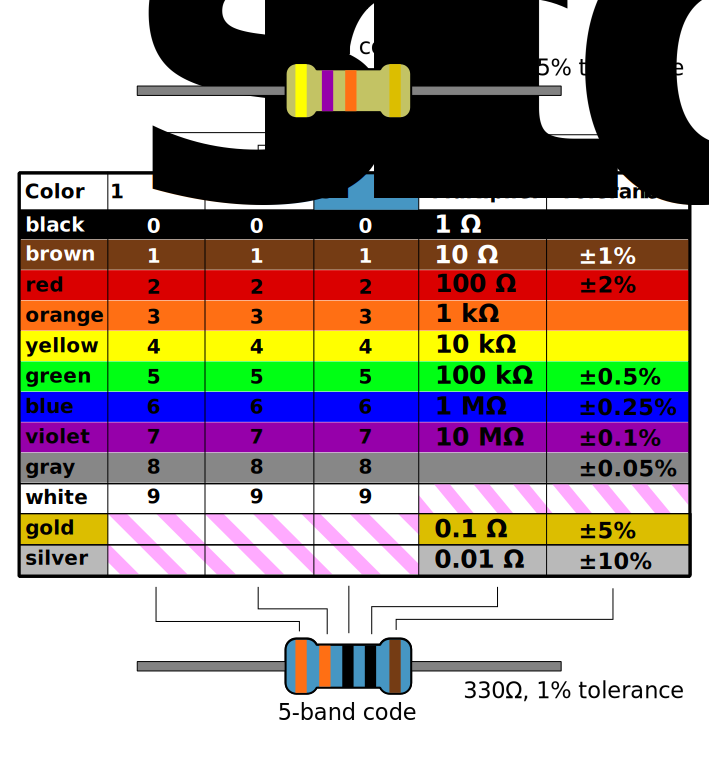
\includegraphics[scale=0.60]{resistorchart.png}
}
\end{center}
\caption{A resistor value color band chart. The `tolerance' stripe (how close the value is guaranteed to be to the stated value) is on the right side. }
\label{fig:resistorchart}
\end{figure}

%---------------------------


%%%%%%%%%%%%%%%%%%%%%%%%%%%%%%%%%%%%%%%%%%%%%%%%%%%%%%%%%%%%%%%%
\end{document}
%%%%%%%%%%%%%%%%%%%%%%%%%%%%%%%%%%%%%%%%%%%%%%%%%%%%%%%%%%%%%%%%
